%%%%%%%%%%%%%%%%%%%%%%%%%%%%%%%%%%%%%%%%%%%%%%%
% CHT-20 Template / Guide For Authors. 
%%%%%%%%%%%%%%%%%%%%%%%%%%%%%%%%%%%%%%%%%%%%%%%
\documentclass[12pt]{CHT-20}
\usepackage{CHT-20}
\usepackage[utf8]{inputenc}
\usepackage{amsmath}
\usepackage{latexsym}
\usepackage{graphicx}
\usepackage{color}
\usepackage{geometry}
\usepackage{empheq}
\usepackage{tikz}
\usepackage{pgfplots}
\usepackage{amsfonts}
\usepackage{commath}
\usepackage{gensymb}
\usepackage{float}
\usepackage{multirow}
%\usepackage{hyperref}
\usepackage{indentfirst}
\usepackage{empheq}
%\usepackage{mathptmx}
\usepackage{amssymb}
\usepackage{cancel}
\usepackage{bm}
\usepackage{siunitx}
\usepackage{tcolorbox}
\usepackage{filecontents}
\usepackage{setspace}
\usepackage[font=small, labelfont=bf]{caption}
\usepackage{enumerate}
\usepackage{nccmath}
\usepackage{booktabs}
\usepackage{wasysym}
\usepackage{xcolor}
\usepackage{fancyhdr}
\usepackage{lastpage}
\usetikzlibrary{shapes.geometric,calc}
\pgfplotsset{compat=1.4}
% \addtolength{\oddsidemargin}{-.875in}
% \addtolength{\evensidemargin}{-.875in}
% \addtolength{\textwidth}{1.75in}
% 
% \addtolength{\topmargin}{-.875in}
% \addtolength{\textheight}{1.75in}
\pgfplotsset{compat=newest} % Allows to place the legend below plot
\usepgfplotslibrary{units} % Allows to enter the units nicely
% Some/most Computer Society conferences require the compsoc mode option,
% but others may want the standard conference format.
%
% If IEEEtran.cls has not been installed into the LaTeX system files,
% manually specify the path to it like:
% \documentclass[conference,compsoc]{../sty/IEEEtran}
%\setlength\extrarowheight{3pt}

\newcommand{\graficoctc}[4]{%
	\centering
	%\begin{minipage}[t][6cm][c]{4.5cm}				
	\begin{tikzpicture}[scale=0.81]
	\begin{axis}[
	axis lines=left,
	%/pgf/number format/1000 sep={.},/pgf/number format/use comma,
	%		xmin = 0,
	%		xmax = 0.04,
	%		ymin = 310,
	%		ymax = 340,
	%		restrict y to domain=-500:2000,
	scaled x ticks = false,
	scaled y ticks = false,
	x tick label style={/pgf/number format/fixed},
	y tick label style={/pgf/number format/fixed},
	xtick = {0, 0.01, 0.02, 0.03, 0.04},
	anchor=east,  
	width=9cm,
	height=7cm,
	label style={font=\footnotesize},
	xlabel = $x$(m),
	xlabel style={at={(1.2, 0)}, anchor = east},
	ylabel= $h_c$ (W/$\text{m}^2$\celsius),		
	ylabel style={rotate=-90, at={(-0.1, 1)}, anchor = south west}]
	\pgfplotstableread{../data/conductance_#2.dat} 
	\teff
	\addplot[color=black, line width=1.2pt] table from \teff;
	\pgfplotstableread{calculated_ctc_interface_#1_conductance_#2_stdev_00.dat} 
	\teff
	\addplot[only marks, color=blue,mark=o,mark options={mark size=1.2pt}] table from \teff;
	\pgfplotstableread{calculated_ctc_interface_#1_conductance_#2_stdev_01.dat} 
	\teff
	\addplot[only marks,color=red,mark=square,mark options={mark size=1.2pt}] table from \teff;
	\pgfplotstableread{calculated_ctc_interface_#1_conductance_#2_stdev_05.dat} 
	\teff
	\addplot[only marks,color=gray,mark=triangle,mark options={mark size=1.2pt}] table from \teff;
	\end{axis}
	\end{tikzpicture}
	%\caption*{(#4) Profile #3}
	%\end{minipage}
}%

\newcommand{\graficoctcunc}[4]{%
	\centering
	%\begin{minipage}[t][6cm][c]{4.5cm}				
	\begin{tikzpicture}[scale=0.81]
	\begin{axis}[
	axis lines=left,
	%/pgf/number format/1000 sep={.},/pgf/number format/use comma,
	%		xmin = 0,
	%		xmax = 0.04,
	%		ymin = 310,
	%		ymax = 340,
	%		restrict y to domain=-500:2000,
	scaled x ticks = false,
	scaled y ticks = false,
	x tick label style={/pgf/number format/fixed},
	y tick label style={/pgf/number format/fixed},
	xtick = {0, 0.01, 0.02, 0.03, 0.04},
	anchor=east,  
	width=9cm,
	height=7cm,
	label style={font=\footnotesize},
	xlabel = $x$(m),
	xlabel style={at={(1.2, 0)}, anchor = east},
	ylabel= $h_c$ (W/$\text{m}^2$\celsius),		
	ylabel style={rotate=-90, at={(-0.1, 1)}, anchor = south west}]
	\pgfplotstableread{../data/conductance_#2.dat} 
	\teff
	\addplot[color=black, line width=1.2pt] table from \teff;
	\pgfplotstableread{uncert/calculated_ctc_interface_#1_conductance_#2_stdev_00.dat} 
	\teff
	\addplot[only marks, color=blue,mark=o,mark options={mark size=1.2pt}] table from \teff;
	\pgfplotstableread{uncert/calculated_ctc_interface_#1_conductance_#2_stdev_01.dat} 
	\teff
	\addplot[only marks,color=red,mark=square,mark options={mark size=1.2pt}] table from \teff;
	\pgfplotstableread{uncert/calculated_ctc_interface_#1_conductance_#2_stdev_05.dat} 
	\teff
	\addplot[only marks,color=gray,mark=triangle,mark options={mark size=1.2pt}] table from \teff;
	\end{axis}
	\end{tikzpicture}
	%\caption*{(#4) Profile #3}
	%\end{minipage}
}%

\pnumber{CHT-20-309}
\ptitle{ESTIMATION OF THERMAL CONTACT CONDUCTANCE ON IRREGULAR INTERFACES USING THE RECIPROCITY FUNCTIONAL APPROACH}


\author[*,\S]{Guilherme C. de Freitas}
\author[*,\dag]{Marcelo J. Colaço}

\affil[*]{Department of Mechanical Engineering, POLI/COPPE, Federal University of Rio de Janeiro, Brazil}
%\affil[**]{Department of Mechanical Engineering, POLI/COPPE, Federal University of Rio de Janeiro, Brazil}
\affil[ \S]{Correspondence author. Email: guifrei@coppe.mecanica.ufrj.br}
\affil[ \dag]{Correspondence author. Email: colaco@ufrj.br}

\pabstract{In some industry applications, such as evaluation of the quality of contact between
	material bodies, or identification of discontinuities or cracks inside a homogeneous body, it
	is required the estimation of a thermophysical parameter known as thermal contact
	conductance. In order to calculate this parameter, one has to determine the distribution of
	temperature discontinuities along the contact surface, as well as the heat flux across that
	surface; the ratio of these two parameters gives the desired thermal contact conductance.
	However, the task of estimating those parameters presents difficulties because the
	methods employed may demand direct measurements, usually obtained by intrusive
	means; or they may demand a detailed description of the surfaces in contact, which is not
	always available. Several strategies have been developed, eventually falling into either of
	the features just described. Recently, some works conducted by our group have been able
	to address these issues by applying the Reciprocity Functional approach, leading to a non-intrusive and non-iterative method for estimation of the thermal contact conductance. In this
	approach, a set of auxiliary problems are introduced and their solutions are used to
	assemble closed-form expressions for estimating the temperature discontinuities and
	heat flux across the contact interface. This method has been succesfully employed in the
	estimation of thermal contact conductances along planar contact interfaces inside composites
	having a rectangular cross-section. This paper aims to extend the application of the
	Reciprocity Functionals to a more general class of problems, in which the contact
	interfaces have arbitrary, non-regular shapes, being the planar contact interface a
	particular case. The results obtained show how this approach is capable of recovering the
	distributions of temperature discontinuities and heat flow across the contact interface in a
	fast and effective fashion. This paper also presents a stopping criteria for the summation series developed in the method, which provide the aforementioned quantities. The influence of the uncertainty in the location of the contact interface is also analyzed in this paper.}

\begin{document}

\maketitle

\makeabstract

\section*{Introduction}

If heat transfer takes place through a common boundary between two bodies in physical contact, a discontinuity in the temperature profile is observed across the contact interface, which indicates that the thermal contact is not perfect there. The ratio of the heat flux per area unit to the temperature drop, both evaluated at that interface, is called \textit{thermal contact conductance} (TCC):

\begin{equation}
h_c = \frac{q_c}{\Delta T_c} \label{definicao_1}
\end{equation}

where $q_c$ is the heat flux and $\Delta T_c$ is the temperature jump, both evaluated across the contact interface. 

An equivalent definition of the TCC may be established upon the analysis of the associated heat conduction problem, by means of the boundary conditions evaluated on the contact interface. Thus, if $T_1$ and $T_2$ are the temperature fields in each of the solids whose contact interface is designated by $\Gamma$, and  $k_1$ and $k_2$ are their respective thermal conductivities, then energy balance allows the following relation:

\begin{equation}
-k_1\frac{\partial T_1}{\partial \mathbf{n}_1}\bigg|_\Gamma
=
h_c(T_1 - T_2)_\Gamma
=
k_2\frac{\partial T_2}{\partial \mathbf{n}_2}\bigg|_\Gamma \label{definicao_2}
\end{equation}
which leads to

\begin{equation}
h_c = \frac{-k_1\displaystyle\frac{\partial T_1}{\partial \mathbf{n}_1}\bigg|_\Gamma}{(T_1 - T_2)_\Gamma} = \frac{k_2\displaystyle\frac{\partial T_2}{\partial \mathbf{n}_2}\bigg|_\Gamma}{(T_1 - T_2)_\Gamma} \label{definicao_3}
\end{equation}

The TCC may be seen as a parameter to evaluate the quality of the contact between two solid bodies. In extreme cases, the TCC vanishes on perfect thermally insulated regions along the contact interface, since the heat flux on the numerator in \eqref{definicao_1} will be zero, whereas an infinite value for TCC will be found where the contact itself is perfect, for which the temperature jump on the denominator in \eqref{definicao_1} will be zero. The TCC may also be useful for evaluating the presence of discontinuities or cracks inside heterogeneous materials; in fact, temperature jumps appear at those regions and the temperature fields measured on the external boundaries of the material will show values different from the expected ones if those discontinuities did not exist. Some examples of the necessity of calculating or estimating the TCC may be found in aerodynamics \citep{artigo_aerospacial}, microelectronics \citep{artigo_snaith} or heat exchanger projects \citep{artigo_huang}. 

Some measuring methods developed for estimating the TCC usually demand knowing details of the surfaces in contact, as well as evaluations of the temperature and heat flux inside the bodies in contact, either \textit{in loco} or through some kind of regression from measurements at inner points, resulting in complex or intrusive experimental assemblies \citep{artigo_fenech, tese_mikic, artigo_beck, artigo_salgon}. Still, due to its special features, this problem may be classified as an Inverse Heat Conduction Problem (abbreviated as IHCP); in that case, the distribution of TCC across the contact interface may be considered as the unknown function to be estimated, by means of the definition \eqref{definicao_1}. In any case, the distributions of heat flux and temperature jumps across the contact interface, which are necessary for estimation of TCC from \eqref{definicao_1}, still need to be measured or calculated.

The concept of Reciprocity Functional (RF), introduced by \cite{artigo_andrieux}, has been applied in recent researches on indirect evaluation of temperature jumps and heat flux distributions across contact interfaces \citep{reciproc_3, artigo_colaco_2, artigo_colaco_3, artigo_abreu_2,artigo_abreu_3, artigo_padilha_2}. These works resulted in the development of non-intrusive, non-iterative, and computationally more efficient approaches for estimating the TCC. However, these techniques have been applied to regular geometrical configurations, such as rectangular or circular-shaped cross section contact interfaces. Nevertheless, the analytical development envolving the use of the RF approach is not restricted to any particular geometry, and may be expanded to more compreehensive configurations.

This paper presents and discusses the problem of estimating the TCC between two solid bodies in contact, considering that the contact interface is not necessarily regular. The starting point is the work developed by \cite{reciproc_3}, who studied the specific case in which the contact interface is planar and horizontal, given that both bodies have a rectangular cross section shape. The auxiliary problems, which provide the necessary functions to be used in the RF approach, were solved using the Method of Fundamental Solutions. \cite{artigo_padilha_3}, by means of the Classic Integral Transform Technique (CITT)\citep{livro_integral_transforms_cotta}, deduced an algebraic expression to estimate the TCC for this particular case model.

For the sake of generality, the contact interface will have a curvilinear format, represented by an equation of the form $y = w(x)$, and the assembly composed by the two bodies in contact will have a rectangular cross section shape. Under these conditions, the original test problem \citep{reciproc_3} may be considered as a special case of the present work, in which the function $w(x)$ will assume a constant value. 

\section*{Physical problem}

The two-dimensional, steady-state problem considered in this paper, whose physical assembly is shown in Figure \ref{fig2}, is based on the configuration proposed by \cite{reciproc_3} and \cite{artigo_abreu_3}. It consists of a specimen $\Omega$ having a rectangular shaped cross section of width $a$ and height $b$, composed by two isotropic bodies $\Omega_1$ and $\Omega_2$, having thermal conductivities $k_1$ and $k_2$ respectively. It is assumed that there is a TCC varying with the position along the contact interface $\Gamma$ between the bodies, represented by the function $h_c(x, y)$.

The lateral boundary surfaces $\Gamma_1$ and $\Gamma_2$ from both layers are kept thermally insulated; the bottom surface $\Gamma_\infty$ is subject to a prescribed temperature, and the upper surface $\Gamma_0$ is subject to a prescribed heat flux $q$. The intersection between any plane parallel to the coordinate plane $xy$ and the interface $\Gamma$ generates a curve described by an equation of the form $y = w(x)$. Since the coordinates $x$ and $y$ are directly related along the interface, the TCC will depend only on $x$, that is, $h_c(x, y) \equiv h_c(x)$.

\begin{figure}[H]
	\begin{center}
		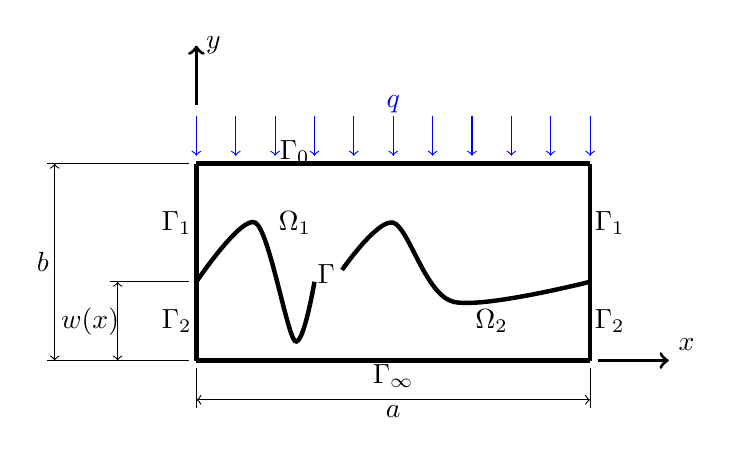
\begin{tikzpicture}[scale=0.5]
		
		\draw [ultra thick] (0, 0) -- (10, 0);
		%\draw [ultra thick] (0, 2) -- (7, 2);
		%\draw [ultra thick] (8, 2) -- (10, 2);
		\draw [ultra thick] plot [smooth] coordinates {(0, 2) (1.5, 3.5) (2.5, 0.5) (3, 2)};
		\draw [ultra thick] plot [smooth] coordinates {(3.7, 2.3) (5, 3.5) (6.5, 1.5) (10, 2)};
		\draw [ultra thick] (0, 5) -- (10, 5);
		\draw [ultra thick] (0, 0) -- (0, 5);
		\draw [ultra thick] (10, 0) -- (10, 5);
		
		\draw (2.5, 3.5) node {$\Omega_1$};
		\draw (7.5, 1) node {$\Omega_2$};	
		\draw (3.3, 2.2) node {$\Gamma$};
		\draw (-0.5, 3.5) node {$\Gamma_1$};
		\draw (-0.5, 1) node {$\Gamma_2$};
		\draw (10.5, 3.5) node {$\Gamma_1$};
		\draw (10.5, 1) node {$\Gamma_2$};
		\draw (5, -0.4) node {$\Gamma_\infty$};
		\draw (2.5, 5.3) node {$\Gamma_0$};
		\draw [blue](5, 6.5) node {$q$};
		\draw (5, -1.3) node {$a$};
		\draw (-3.9, 2.5) node {$b$};
		\draw (-2.7, 1) node {$w(x)$};
		
		\node [above right] at (12, 0) {$x$};
		\node [right] at (0, 8) {$y$};
		
		\draw [->, blue] (0, 6.2) -- (0, 5.2);
		\draw [->, blue] (1, 6.2) -- (1, 5.2);
		\draw [->, blue] (2, 6.2) -- (2, 5.2);
		\draw [->, blue] (3, 6.2) -- (3, 5.2);
		\draw [->, blue] (4, 6.2) -- (4, 5.2);
		\draw [->, blue] (5, 6.2) -- (5, 5.2);
		\draw [->, blue] (6, 6.2) -- (6, 5.2);
		\draw [->, blue] (7, 6.2) -- (7, 5.2);
		\draw [->, blue] (8, 6.2) -- (8, 5.2);
		\draw [->, blue] (9, 6.2) -- (9, 5.2);
		\draw [->, blue] (10, 6.2) -- (10, 5.2);
		
		\draw [->, very thick] (10.2,0) -- (12,0);
		\draw [->, very thick] (0, 6.5) -- (0,8);
		
		\draw [-] (0, -0.2) -- (0, -1.2);
		\draw [-] (10, -0.2) -- (10, -1.2);
		\draw [<->] (0, -1) -- (10, -1);
		
		\draw [-] (-0.2, 0) -- (-3.8, 0);
		\draw [-] (-0.2, 5) -- (-3.8, 5);
		\draw [-] (-0.2, 2) -- (-2.2, 2);
		\draw [<->] (-3.6, 0) -- (-3.6, 5);
		\draw [<->] (-2.0, 0) -- (-2.0, 2);
		
		\end{tikzpicture}
		\caption{Schematic representation of the physical problem}
		\label{fig2}
	\end{center}
\end{figure}

The formulation of the direct steady-state heat conduction problem is given as follows:
\begin{subequations}
	\begin{alignat}{2}
	& \nabla^2 T_1 = 0 \quad\quad\quad\quad && \text{ in } \Omega_1 \label{harm_T1} \\ \nonumber \\
	& -k_1 \frac{\partial T_1}{\partial\mathbf{n}_1} = q && \text{ on } \Gamma_0  \label{cc_T1_2} \\  \nonumber \\
	& \frac{\partial T_1}{\partial \mathbf{n}_1} = 0 && \text{ on }  \Gamma_1 \label{cc_T1_1} \\  \nonumber \\
	& -k_1 \frac{\partial T_1}{\partial\mathbf{n}_1} = h_c(T_1-T_2) \quad\quad\quad\quad && \text{ on }  \Gamma \label{cc_grad_T1} \\  \nonumber \\
	& \nabla^2 T_2 = 0 && \text{ in }  \Omega_2 \label{harm_T2} \\  \nonumber \\
	& \frac{\partial T_2}{\partial \mathbf{n}_2} = 0 && \text{ on }  \Gamma_2 \label{cc_T1_3} \\ \nonumber \\
	& T_2 = 0 && \text{ on }  \Gamma_\infty \label{cc_T1_4} \\  \nonumber \\
	& k_2\frac{\partial T_2}{\partial\mathbf{n}_2} = - k_1\frac{\partial T_1}{\partial\mathbf{n}_1} && \text{ on }  \Gamma \label{cc_T1_5}
	\end{alignat}
\end{subequations}

In the above equations, $T_1$ and $T_2$ are the temperature fields corresponding to domains $\Omega_1$ and $\Omega_2$ respectively, and the normal unitary vectors $\mathbf{n}_1$ and $\mathbf{n}_2$ point outward the corresponding domains. Particularly at the contact interface $\Gamma$, it can be observed that $\mathbf{n}_1 = -\mathbf{n}_2$.

\section*{Inverse problem}

The inverse problem considered in this work is concerned with the estimation of the function $h_c(x)$ by means of the equation \eqref{definicao_3} on the contact interface $\Gamma$ between the two bodies $\Omega_1$ and $\Omega_2$, according to the physical arrangement illustrated in Figure \ref{fig2}. The estimation will be performed by using temperature measurements $Y = T(\Gamma_0)$ taken, for example, by a thermographic camera on interface $\Gamma_0$. Both surfaces $\Gamma_1$ and $\Gamma_2$ will be kept thermically insulated, and the bottom surface $\Gamma_\infty$ will be subjected to the same prescribed temperature as in the direct problem. The heat flux $q_c(x) = -k_1\frac{\partial T_1}{\partial \mathbf{n}_1}$ and the temperature jump $\Delta T_c(x) = T_1 - T_2$, both evaluated at the contact interface $\Gamma$, will be indirectly estimated by defining and solving two separated auxiliary problems, as proposed by \cite{reciproc_3}.

\section*{Application of the reciprocity functional}

Based on the idea of reciprocity functional gap developed by \cite{artigo_andrieux}, \cite{reciproc_3} introduced the concept of Reciprocity Functional (RF) through the following expression:
\begin{align}
\Re(F) = \int_{\Gamma_0}\left[\left(\frac{-q}{k_1}\right)F - Y\frac{\partial F}{\partial\mathbf{n_1}}\right]d\Gamma_0
\label{def_funcional_reciprocidade}
\end{align}
where $F$ is a harmonic function defined over $\Omega_1$, and $Y$ represents the measured temperatures along the upper boundary surface $\Gamma_0$.

\cite{reciproc_3} formulated two diffusive problems for determining two classes of auxiliary functions $F_1$ and $G_1$, over the same domain $\Omega_1$. Combining the direct problem expressed in \eqref{harm_T1}--\eqref{cc_T1_5} with the auxiliary problems and their boundary conditions, and applying Green's second theorem, they were able to demonstrate the following identities, which relate the temperature jump and the heat flux at the inaccessible interface $\Gamma$ to the measured temperatures $Y$ along the external surface $\Gamma_0$:
\begin{align}
k_1\int_{\Gamma_0}\left[\left(\frac{-q}{k_1}\right)\right. & \left.F_1 - Y\frac{\partial F_1}{\partial\mathbf{n_1}}\right]d\Gamma_0
= \int_\Gamma k_1 \frac{\partial F_1}{\partial\mathbf{n_1}}\left(T_1 - T_2\right)d\Gamma
\label{identidade_T} \\ \nonumber \\
k_1\int_{\Gamma_0}\left[\left(\frac{-q}{k_1}\right)\right. & \left.G_1 -  Y\frac{\partial G_1}{\partial\mathbf{n_1}}\right]d\Gamma_0
= \int_\Gamma -k_1 G_1 \frac{\partial T_1}{\partial\mathbf{n_1}}d\Gamma
\label{identidade_q}
\end{align}

Now let $k_1 \frac{\partial F}{\partial\mathbf{n_1}}$, $T_1 - T_2$, $G$ and $-k_1 \frac{\partial T_1}{\partial\mathbf{n_1}}$ belong to a linear space of functions $L^2(\Gamma)$, and let the inner product in this linear space be defined as:
\begin{align}
\langle f_1, f_2\rangle_{L^2(\Gamma)} = \int_\Gamma f_1(\Gamma) f_2(\Gamma) d\Gamma \label{definicao_innner_product}
\end{align} 

By rasing two families of auxiliary functions $F_{1,j}, j=1,2,\ldots N_1$ and $G_{1,j}, j=1,2,\ldots N_2$ from the corresponding auxiliary problems, and using the definition of inner product in \eqref{definicao_innner_product}, as well as the definition of the RF in \eqref{def_funcional_reciprocidade}, expressions \eqref{identidade_T} and \eqref{identidade_q} may be rewritten as:
\begin{align}
& k_1 \Re(F_{1,j})
=
\left\langle \left[T_1 - T_2\right]_\Gamma, \beta_j\right\rangle _{L^2(\Gamma)}
\label{identidade_T_inner} \\ \nonumber \\
& k_1 \Re(G_{1,j})
=
\left\langle  -k_1 \frac{\partial T_1}{\partial\mathbf{n_1}}\bigg|_\Gamma, \gamma_j\right\rangle _{L^2(\Gamma)}
\label{identidade_q_inner}
\end{align}
where
\begin{align}
& \beta_j = k_1 \frac{\partial F_{1,j}}{\partial\mathbf{n_1}}\bigg|_\Gamma \label{expressao_define_beta} \\ \nonumber \\
& \gamma_j = G_{1,j}\big|_\Gamma \label{expressao_define_gamma}
\end{align}

Assuming that $\beta_j, j=1,2,\ldots N_1$ and $\gamma_j, j=1,2,\ldots N_2$ form two sets of orthonormal functions, they defined two linear subspaces over which $T_1 - T_2$ and $-k_1 \frac{\partial T_1}{\partial\mathbf{n_1}}$ may be ortogonally projected, that is:
\begin{align}
& [T_1 - T_2]_\Gamma \approx \sum_{j=1}^{N_1} \left\langle  \left[T_1 - T_2\right]_\Gamma, \beta_j \right\rangle_{L^2(\Gamma)} \beta_j \\ \nonumber \\
& - k_1 \frac{\partial T_1}{\partial\mathbf{n_1}}\bigg|_\Gamma \approx \sum_{j=1}^{N_2} \left\langle  -k_1 \frac{\partial T_1}{\partial\mathbf{n_1}}\bigg|_\Gamma, \gamma_j \right\rangle_{L^2(\Gamma)} \gamma_j
\end{align}

Applying identities \eqref{identidade_T_inner} and \eqref{identidade_q_inner} to the above equations, and assuming that the orthogonal projections represent the corresponding functions in a reasonable manner, the following relations can be written:
\begin{align}
& [T_1 - T_2]_\Gamma = \sum_{j=1}^{N_1} k_1 \Re(F_{1,j}) \beta_j \label{resultado_1} \\ \nonumber \\
& - k_1 \frac{\partial T_1}{\partial\mathbf{n_1}}\bigg|_\Gamma = \sum_{j=1}^{N_2} k_1 \Re(G_{1,j}) \gamma_j \label{resultado_2}
\end{align}

The substitution of these results into the definition of the TCC \eqref{definicao_3} leads to:
\begin{align}
& h_c(x) % = \frac{- k_1 \displaystyle\frac{\partial T_1}{\partial\mathbf{n_1}}\bigg|_\Gamma}{[T_1 - T_2]_\Gamma} 
= \frac{\displaystyle\sum_{j=1}^{N_2} \Re(G_{1,j}) \gamma_j(x)}{\displaystyle\sum_{j=1}^{N_1} \Re(F_{1,j}) \beta_j(x)}
\label{equacao_definicao_f_r}
\end{align}

The expression \eqref{equacao_definicao_f_r} allows the estimation of the TCC distribution along the contact interface $\Gamma$, by knowing the distribution of temperatures $Y$ measured along the external interface $\Gamma_0$, thus eliminating the previous need of knowing internal characteristics of the composite body, confirming the non-intrusive feature of the method. The families of functions $F_{1, j}$ and $G_{1, j}$, and the integrals that provide the Reciprocity Functional values envolving these functions, need to be calculated just once for a certain geometric and thermophysical characterization of the problem, so that the method is also non-iterative.

\section*{Formulation and solution of the auxiliary problem}
\subsection*{First auxiliary problem: estimation of the temperature jump at the contact interface}

Let $F_{1,j}$ and $F_{2,j}$ be two families of harmonic functions, defined over the domains $\Omega_1$ and $\Omega_2$ respectively, and let $\psi_j(x), j=1,2,\ldots N_1$ be a family of linear independent functions. The first auxiliary problem, as proposed by \cite{artigo_abreu_3}, may be defined as follows:
\begin{subequations}
	\begin{alignat}{2}
	& \nabla^2 F_{1,j} = 0 \quad\quad\quad\quad\quad && \text{ in } \Omega_1 \label{funcao_F_harm_T1} \\ \nonumber \\
	& F_{1,j} = \psi_j && \text{ on } \Gamma_0  \label{funcao_F_cc_T1_2} \\ \nonumber \\
	& \frac{\partial F_{1,j}}{\partial \mathbf{n}_1} = 0 && \text{ on }  \Gamma_1 \label{funcao_F_cc_T1_1} \\  \nonumber \\
	& F_{1,j} = F_{2, j} \quad\quad\quad\quad\quad\quad\quad\quad && \text{ on }  \Gamma \label{funcao_F_cc_grad_T1} \\ \nonumber \\
	& \nabla^2 F_{2,j} = 0 && \text{ in }  \Omega_2 \label{funcao_F_harm_T2} \\ \nonumber \\
	& \frac{\partial F_{2,j}}{\partial \mathbf{n}_2} = 0 && \text{ on }  \Gamma_2 \label{funcao_F_cc_T1_3} \\ \nonumber \\
	& F_{2,j} = 0 && \text{ on }  \Gamma_\infty \label{funcao_F_cc_T1_4} \\ \nonumber \\
	& k_2\frac{\partial F_{2, j}}{\partial\mathbf{n}_2} = - k_1\frac{\partial F_{1,j}}{\partial\mathbf{n}_1} && \text{ on }  \Gamma \label{funcao_F_cc_T1_5}
	\end{alignat}
\end{subequations}

\subsection*{Second auxiliary problem: estimation of the heat flux at the contact interface}

Let $G_{1,j}$ be a family of harmonic functions, defined over the domain $\Omega_1$, and let $\phi_j(x), j=1,2,\ldots N_2$ be a family of linear independent functions. The second auxiliary problem, as proposed by \cite{artigo_abreu_3}, may be defined as follows:
\begin{subequations}
	\begin{alignat}{2}
	& \nabla^2 G_{1,j} = 0 \quad\quad\quad\quad\quad && \text{ in } \Omega_1 \label{funcao_G_harm_T1} \\  \nonumber \\
	& G_{1,j} = \phi_j && \text{ on } \Gamma_0  \label{funcao_G_cc_T1_2} \\ \nonumber \\
	& \frac{\partial G_{1,j}}{\partial \mathbf{n}_1} = 0 && \text{ on }  \Gamma_1 \label{funcao_G_cc_T1_1} \\  \nonumber \\
	& \frac{\partial G_{1,j}}{\partial\mathbf{n}_1} = 0 \quad\quad\quad\quad\quad\quad\quad\quad && \text{ on }  \Gamma \label{funcao_G_cc_grad_T1}
	\end{alignat}
\end{subequations}

\subsection*{Solution of the auxiliary problems using CITT}
The Classic Integral Transform Technique (CITT) provides a systematic and efficient approach for solving linear diffusive problems envolving nonhomogeneous terms in the differential equations or in the boundary conditions \citep{livro_integral_transforms_cotta}, and was employed by \cite{artigo_padilha_3} for the solution of the auxiliary problems formulated in the previous subsections, specifically for the case of the planar horizontal contact interface. Since the current study comprises a more general configuration, still keeping the basic thermophysical and geometrical characteristics, that method was a natural choice for solving its corresponding auxiliary problems.

In order to solve equations \eqref{funcao_F_harm_T1} to \eqref{funcao_F_cc_T1_5} and \eqref{funcao_G_harm_T1} to \eqref{funcao_G_cc_grad_T1} by the CITT method, it is necessary to define the following integral transforms and inversion formulas \citep{livro_integral_transforms_cotta} in the $x$-direction, where the boundary conditions are homogeneous:
\begin{itemize}
	\item Functions $F_{1, j}$ and $F_{2, j}$:
	\begin{subequations}
		\begin{align}
		& \bar{F}_{1,j,m}(y) = \int_0^a F_{1, j}(x, y) X(\mu_m, x) dx \label{definicao_da_transf_F1}  \\ \nonumber \\
		& F_{1, j}(x, y) = \sum_{m=0}^\infty \frac{X(\mu_m, x)}{N(\mu_m)}\bar{F}_{1,j,m}(y) \label{definicao_da_transf_inv_F1}	 \\ \nonumber \\
		& \bar{F}_{2,j,m}(y) = \int_0^a F_{2, j}(x, y) X(\mu_m, x) dx \label{definicao_da_transf_F2}  \\ \nonumber \\
		& F_{2, j}(x, y) = \sum_{m=0}^\infty \frac{X(\mu_m, x)}{N(\mu_m)}\bar{F}_{2,j,m}(y) \label{definicao_da_transf_inv_F2}	
		\end{align}
	\end{subequations}
	\item Functions $G_{1, j}$:
	\begin{subequations}
		\begin{align}
		& \bar{G}_{1,j,m}(y) = \int_0^a G_{1, j}(x, y) X(\mu_m, x) dx \label{definicao_da_transf_G1}  \\ \nonumber \\
		& G_{1, j}(x, y) = \sum_{m=0}^\infty \frac{X(\mu_m, x)}{N(\mu_m)}\bar{G}_{1,j,m}(y) \label{definicao_da_transf_inv_G1}		
		\end{align}
	\end{subequations}
\end{itemize}

In the above equations, $X(\mu_m, x)$ are the eigenfunctions of the following associate eigenvalue problem \citep{livro_integral_transforms_cotta}:
\begin{subequations}
	\begin{alignat}{2}
	& \frac{d^2 X(\mu_m, x)}{d x^2} + \mu_m^2 X(\mu_m, x) = 0, && 0 < x < a \label{problema_vc_1a} \\ \nonumber \\
	& \frac{d X(\mu_m, x)}{d x} = 0 && x = 0 \label{problema_vc_1b} \\ \nonumber \\
	& \frac{d X(\mu_m, x)}{d x} = 0 && x = a \label{problema_vc_1c}
	\end{alignat}
\end{subequations}
and the norm $N(\mu_m)$ is given as \citep{livro_integral_transforms_cotta}:
\begin{align}
N(\mu_m) = \left\lbrace
\begin{array}{ll}
a, \quad\quad\quad\quad & m = 0 \\ \\
\displaystyle\frac{a}{2}, & m = 1,2,3,\ldots
\end{array}
\right. \label{valor_integral_norm}
\end{align}

The solution of \eqref{problema_vc_1a} is given as \citep{livro_integral_transforms_cotta}:
\begin{align}
& X(\mu_m, x) = \left\lbrace
\begin{array}{ll}
1, & m = 0 \\ \\
\cos \mu_m x, & m = 1,2,3,\ldots
\end{array}
\right . \label{definicao_das_autofuncoes}
\end{align}
where the eigenvalues $\mu_m$ are given as \citep{livro_integral_transforms_cotta}:
\begin{align}
\mu_m = \left\lbrace
\begin{array}{ll}
0, \quad\quad\quad\quad & m = 0 \\ \\
\displaystyle\frac{m\pi}{a}, & m = 1,2,3,\ldots
\end{array}
\right.
\label{eigenvals}
\end{align}

Applying the integral transform to the partial differential equations \eqref{funcao_F_harm_T1}, \eqref{funcao_F_harm_T2} and \eqref{funcao_G_harm_T1}, the dependency on $x$ is eliminated, and the following ordinary equations in $y$ are obtained:
\begin{align}
& \frac{d^2 \bar{F}_{1,j,m}(y)}{d y^2}
-
\mu_m^2 \bar{F}_{1,j,m}(y) = 0 \label{eq_dif_ord_F1} \\ \nonumber \\
& \frac{d^2 \bar{F}_{2,j,m}(y)}{d y^2}
-
\mu_m^2 \bar{F}_{2,j,m}(y) = 0 \label{eq_dif_ord_F2} \\ \nonumber \\
& \frac{d^2 \bar{G}_{1,j,m}(y)}{d y^2}
-
\mu_m^2 \bar{G}_{1,j,m}(y) = 0 \label{eq_dif_ord_G1}
\end{align}

Applying the integral transform to the boundary conditions \eqref{funcao_F_cc_T1_2}, \eqref{funcao_F_cc_T1_4} and \eqref{funcao_G_cc_T1_2}, and using the resulting conditions for solving the above differential equations, the following general solutions may be found \citep{livro_boyce}:
\begin{align}
& \bar{F}_{1,j,m}(y) = \mathbb{A}_{j,m} \frac{\sinh\mu_m (b - y)}{\sinh\mu_m b} +	\bar{\psi}_{j, m}\frac{\sinh\mu_m y}{\sinh\mu_m b} \label{solucao_temporaria_F1} \\ \nonumber \\
& \bar{F}_{2,j,m}(y) = \mathbb{D}_{j,m}\frac{\sinh\mu_m y}{\sinh\mu_m b} \label{solucao_temporaria_F2} \\ \nonumber \\
& \bar{G}_{1,j,m}(y) = \mathbb{E}_{j,m} \frac{\sinh\mu_m (b - y)}{\sinh\mu_m b} +\bar{\phi}_{j, m}\frac{\sinh\mu_m y}{\sinh\mu_m b} \label{solucao_temporaria_G1}
\end{align}
where $\bar{\psi}_{j, m}$ and $\bar{\phi}_{j, m}$ are the integral transforms of $\psi_j(x)$ and $\phi_j(x)$, and $\mathbb{A}_{j,m}$, $\mathbb{D}_{j,m}$ and $\mathbb{E}_{j,m}$ are constants to be determined.

In order to evaluate those constants, the inverse formulas \eqref{definicao_da_transf_inv_F1}, \eqref{definicao_da_transf_inv_F2} and \eqref{definicao_da_transf_inv_G1} must be substituted into boundary conditions \eqref{funcao_F_cc_grad_T1}, \eqref{funcao_F_cc_T1_5} and \eqref{funcao_G_cc_grad_T1}, and the resulting expressions must be transformed, which leads to an infinite linear system for $\mathbb{A}_{j,m}$ and $\mathbb{D}_{j,m}$ as follows:
\begin{subequations}
	\begin{align}
	& \sum_{m = 0}^\infty \bar{a}_{n,m} \mathbb{A}_{j,m} + \sum_{m = 0}^\infty \bar{b}_{n,m} \mathbb{D}_{j,m} = \bar{c}_{n,j} \label{sistema_para_coeficientes_1}
	\end{align}
	\begin{align}
	& \sum_{m = 0}^\infty \bar{p}_{n,m} \mathbb{A}_{j,m} + \sum_{m = 0}^\infty \bar{q}_{n,m} \mathbb{D}_{j,m} = \bar{r}_{n,,j} \label{sistema_para_coeficientes_2}
	\end{align}
\end{subequations}
and an inifinite linear system for $\mathbb{E}_{j,m}$ as follows:
\begin{align}
& \sum_{m = 0}^\infty \bar{u}_{n,m} \mathbb{E}_{j,m} = \bar{v}_{n,j} \label{sistema_para_coeficientes_3}
\end{align}
where $\bar{a}_{n,m}$, $\bar{b}_{n,m}$, $\bar{c}_{n,j}$, $\bar{p}_{n,m}$, $\bar{q}_{n,m}$, $\bar{r}_{n,j}$, $\bar{u}_{n,m}$ and $\bar{v}_{n,j}$ are constants calculated by the integral transforms of expressions that depend on $w(x)$.

The expressions \eqref{sistema_para_coeficientes_1}, \eqref{sistema_para_coeficientes_2} and \eqref{sistema_para_coeficientes_3} define a set of infinite linear systems. In order to search for an approximate solution to these equations, the infinite sums have to be truncated up to a limiting index $M$:
\begin{subequations}
	\begin{align}
	& \sum_{m = 0}^M \bar{a}_{n,m} \mathbb{A}_{j,m} + \sum_{m = 0}^\infty \bar{b}_{n,m} \mathbb{D}_{j,m} \approx \bar{c}_{n,j} \label{sistema_para_coeficientes_1a}
	\end{align}
	\begin{align}
	& \sum_{m = 0}^M \bar{p}_{n,m} \mathbb{A}_{j,m} + \sum_{m = 0}^\infty \bar{q}_{n,m} \mathbb{D}_{j,m} \approx \bar{r}_{n,,j} \label{sistema_para_coeficientes_2a}
	\end{align}
	\begin{align}
	& \sum_{m = 0}^M \bar{u}_{n,m} \mathbb{E}_{j,m} \approx \bar{v}_{n,j} \label{sistema_para_coeficientes_3a}
	\end{align}
\end{subequations}

The resulting set of linear systems may now be numerically solved to obtain the unknown constants $\mathbb{A}_{j,m}$, $\mathbb{D}_{j,m}$ and $\mathbb{E}_{j,m}$.

The functions $\beta_j(x)$ and $\gamma_j(x)$, required for the estimation of the TCC through equation \eqref{equacao_definicao_f_r}, may be calculated by substituting the previous results in definitions \eqref{expressao_define_beta} and \eqref{expressao_define_gamma}, which gives:
\begin{align}
& \beta_j(x) = \frac{k_1}{\sqrt{1 + w'(x)^2}}\left\lbrace \frac{\mathbb{A}_{j,0} - \bar{\psi}_{j,0}}{ab} +
\right. \nonumber \\
& \frac{2}{a}\sum_{m=1}^M \mu_m  \left[ \mathbb{A}_{j,m}\frac{\scriptstyle\cos\mu_m x\cosh\mu_m v(x) - w'(x)\sin\mu_m x\sinh\mu_m v(x)}{\scriptstyle\sinh\mu_m b} \right. - 
\left. \left. \bar{\psi}_{j, m}\frac{\scriptstyle w'(x)\sin\mu_m x\sinh\mu_m w(x) + \cos\mu_m x\cosh\mu_m w(x)}{\scriptstyle\sinh\mu_m b}\right] \right\rbrace
\label{serie_para_beta}
\end{align}
\begin{align}
\gamma_j(x) = & \frac{\mathbb{E}_{j,0}[b - w(x)] + \bar{\phi}_{j,0}w(x)}{ab} +
\frac{2}{a}\sum_{m=1}^M \left\lbrace\mathbb{E}_{j,m}\frac{\sinh\mu_m [b - w(x)]}{\sinh\mu_m b} + 
\bar{\phi}_{j, m}\frac{\sinh\mu_m w(x)}{\sinh\mu_m b}\right\rbrace \cos\mu_m x
\label{serie_para_gamma}
\end{align} 
where $v(x) = b - w(x)$.

\subsection*{Orthonormalization of the auxiliary functions}
The orthonormality of functions $\beta_j(x)$ and $\gamma_j(x)$ was a prerequisite for applying the expansions \eqref{resultado_1} and \eqref{resultado_2}, which provide the necessary estimatives for the temperature jump and heat flux at the contact interface. At first, this feature cannot be guaranteed for the functions $\beta_j(x)$ and $\gamma_j(x)$ obtained from the previous subsection. However, assuming that the sets of functions $\beta_j(x), j=1,2,\dots, N_1$ and $\gamma_j(x), j=1,2,\dots, N_2$ are linearly independent, it is possible to obtain a new set of functions $\hat{\beta}_j(x)$ and $\hat{\gamma}_j(x)$ fulfilling that condition, by means of the Gram-Schmidt orthonormalization algorithm \citep{livro_axler}:
\begin{align}
\hat{\beta}_j = & \frac{1}{\norm{\nu_j}}\beta_j - \sum_{k=0}^{j-1} \frac{\langle \beta_j, \hat{\beta}_k \rangle_{L^2(\Gamma)}}{\norm{\nu_j}} \hat{\beta}_k, j=1,2,\dots, N_1 \label{termo_beta} \\ \nonumber \\
\hat{\gamma}_j = & \frac{1}{\norm{\upsilon_j}}\gamma_j - \sum_{k=0}^{j-1} \frac{\langle \gamma_j, \hat{\gamma}_k \rangle_{L^2(\Gamma)}}{\norm{\upsilon_j}} \hat{\gamma}_k, j=1,2,\dots, N_2 \label{termo_gamma}
\end{align}
where
\begin{align}
& \nu_j = \beta_j - \sum_{k = 0}^{j - 1} \langle \beta_j, \hat{\beta}_k\rangle_{L^2(\Gamma)}\hat{\beta}_k \\ \nonumber \\
& \upsilon_j = \gamma_j - \sum_{k = 0}^{j - 1} \langle \gamma_j, \hat{\gamma}_k\rangle_{L^2(\Gamma)}\hat{\gamma}_k
\end{align}

Due to the linearity of the auxiliary problems, the corresponding constants $\hat{\mathbb{A}}_{j,m}$ and $\hat{\mathbb{E}}_{j,m}$ may be obtained from an analogous procedure:
\begin{align}
\hat{\mathbb{A}}_{j,m} = & \frac{1}{\norm{\nu_j}} \mathbb{A}_{j,m} - \sum_{k=0}^{j-1} \frac{\langle \beta_j, \hat{\beta}_k \rangle}{\norm{\nu_j}} \hat{\mathbb{A}}_{k,m}, j=1,2,\dots, N_1; m=0,1,2,\ldots,M \label{expressao_relaciona_psi} \\ \nonumber \\
\hat{\mathbb{E}}_{j,m} = & \frac{1}{\norm{\upsilon_j}} \mathbb{E}_{j,m} - \sum_{k=0}^{j-1} \frac{\langle \gamma_j, \hat{\gamma}_k \rangle}{\norm{\upsilon_j}} \hat{\mathbb{E}}_{k,m}, j=1,2,\dots, N_2 ; m=0,1,2,\ldots,M \label{expressao_relaciona_zeta}
\end{align}

Equations \eqref{expressao_relaciona_psi} and \eqref{expressao_relaciona_zeta} are basically recurrence relations that allow the determination of coefficients $\hat{\mathbb{A}}_{j,m}$ and $\hat{\mathbb{E}}_{j,m}$ from coefficients $\mathbb{A}_{j,m}$ and $\mathbb{E}_{j,m}$, which have to be previously calculated as the solution of the linear systems \eqref{sistema_para_coeficientes_1a}, \eqref{sistema_para_coeficientes_2a} and \eqref{sistema_para_coeficientes_3a} (the coefficients $\hat{\mathbb{D}}_{j,m}$ are calculated as a side effect). These new coefficients, when substituted into \eqref{serie_para_beta} and \eqref{serie_para_gamma} at each step of the recurrency process, will provide the functions $\hat{\beta}_j$ and $\hat{\gamma}_j$ that meet the orthonormality criteria. 

From the results obtained so far, it is possible to outline a basic algorithm to determine the functions $\hat{\beta}_j$ and $\hat{\gamma}_j$, which are necessary for estimating the temperature jump and the heat flux across the contact interface, and consequently the thermal contact conductance (see equations \ref{resultado_1}, \ref{resultado_2} and \ref{equacao_definicao_f_r}): 

\begin{enumerate}
	\item Generate the matrices for the linear systems \eqref{sistema_para_coeficientes_1a},  \eqref{sistema_para_coeficientes_2a} and \eqref{sistema_para_coeficientes_3a};
	\item Choose two sets of linearly independent functions, $\psi_j(x), j=0,1,\ldots,N_1$ and $\phi_j(x), j=0,1,\ldots,N_2$;
	\item For each $j$ (ranging from 0 to $N_1$ for $\psi_j(x)$ and 0 to $N_2$ for $\phi_j(x)$):
	\begin{enumerate}	
		\item Calculate the integral transforms $\bar{\psi}_{j,m}$ and $\bar{\phi}_{j,m}, m=0,1,2, \ldots, M$;
		\item Solve the linear system $\mathbf{M}\mathbf{\xi} = \mathbf{b_\psi}$ defined by equations \eqref{sistema_para_coeficientes_1a} and \eqref{sistema_para_coeficientes_2a}, and the linear system $\mathbf{N}\mathbf{\varsigma} = \mathbf{b_\phi}$ defined by equation \eqref{sistema_para_coeficientes_3a}, where $\mathbf{M}$ and $\mathbf{N}$ are the matrices calculated in step 1, and $\mathbf{b_\psi}$ and $\mathbf{b_\phi}$ are the vectors assembled using the values for $\bar{c}_{n,j}$, $\bar{r}_{n,j}$ and $\bar{s}_{n,j}$. The solution vectors $\mathbf{\xi}$ and $\mathbf{\varsigma}$ provide the values for $\mathbb{A}_{j,m}$ and $\mathbb{E}_{j,m}, m=0,1,2, \ldots, M$;
		\item Calculate $\beta_j$ from \eqref{serie_para_beta} using the results from $\mathbb{A}_{j,m}$, and $\gamma_j$ from \eqref{serie_para_gamma} using the results from $\mathbb{E}_{j,m}$;
		\item Calculate $\nu_j$ and $\upsilon_j$:
		\begin{itemize}
			\item If $j = 0$, then $\nu_j = \beta_j$ and $\upsilon_j = \gamma_j$;
			\item If $j \ne 0$, then $\nu_j = \beta_j - \displaystyle\sum_{k = 0}^{j - 1} \langle \beta_j, \hat{\beta}_k\rangle\hat{\beta}_k$ and $\upsilon_j = \gamma_j - \displaystyle\sum_{k = 0}^{j - 1} \langle \gamma_j, \hat{\gamma}_k\rangle\hat{\gamma}_k$;
		\end{itemize}
		\item Calculate $\hat{\mathbb{A}}_{j,m}$ and $\hat{\mathbb{E}}_{j,m}, m=0,1,2, \ldots, M$ from \eqref{expressao_relaciona_psi} and \eqref{expressao_relaciona_zeta};
		\item Calculate $\hat{F}_{1,j}$ using the results for $\hat{\mathbb{A}}_{j,m}$ in \eqref{definicao_da_transf_inv_F1} and \eqref{solucao_temporaria_F1}, and $\hat{G}_{1,j}$ using the results for $\hat{\mathbb{E}}_{j,m}$ in \eqref{definicao_da_transf_inv_G1} and \eqref{solucao_temporaria_G1};
		\item Calculate $\hat{\beta}_j$ from \eqref{serie_para_beta} usando os valores $\hat{\mathbb{A}}_{j,m}$.
	\end{enumerate}
\end{enumerate}


It is important to highlight that the matrices $\mathbf{M}$ and $\mathbf{N}$ from step 1 have to be calculated just once for a particular set of geometrical and thermophysical parameters, because their coefficients do not change along the subsequent calculations. Thus, they can be calculated in advance, and the step 3b can be implemented by means of LU decomposition, which speeds up the numerical computations. It can also be noticed that the step 3 is a recursive process, that is, the results calculated in the $j$-th iteration depend on the results obtained in the previous iterations, namely $j - 1$ down to $0$.

From this point on, for the sake of simplicity, the symbol $\hat{}$ will be dropped, and the coefficients $\mathbb{A}_{j,m}$ and $\mathbb{E}_{j,m}$ will be considered as been calculated after the orthonormality procedure, as well as the functions $F_{1,j}$, $G_{1,j}$, $\beta_j$ and $\gamma_j$.
  
\section*{Analytical formulation for the thermal contact conductance}

Once the family of functions $F_{1,j}$ and $G_{1,j}$ have been determined, they can be replaced into the definition \eqref{def_funcional_reciprocidade}, in order to obtain the following expressions for their respective Reciprocity Functionals:
\begin{align}
\Re(F_{1,j})
& =
-\frac{q}{k_1}\bar{\psi}_{j,0} + \frac{\mathbb{A}_{j,0} - \bar{\psi}_{j,0}}{b} \bar{y}_0 +
\sum_{m=1}^M \mu_m \left(\frac{\mathbb{A}_{j,m}}{\sinh\mu_m b} - \frac{\bar{\psi}_{j, m}}{\tanh\mu_m b}\right)\bar{y}_m
\label{calculo_FR_F1_antes_b} 
\end{align}
\begin{align}
\Re(G_{1,j})
& =
-\frac{q}{k_1}\bar{\phi}_{j,0} + \frac{\mathbb{E}_{j,0} - \bar{\phi}_{j,0}}{b} \bar{y}_0 + 
\sum_{m=1}^M \mu_m \left(\frac{\mathbb{E}_{j,m}}{\sinh\mu_m b} - \frac{\bar{\phi}_{j, m}}{\tanh\mu_m b}\right)\bar{y}_m
\label{calculo_FR_G1_antes_b}
\end{align}
where $\bar{y}_0$ and $\bar{y}_m$ are given as:
\begin{align}
& \bar{y}_0 = \frac{1}{a}\int_0^a Y(x) dx \label{coef_it_0} \\  \nonumber \\
& \bar{y}_m = \frac{2}{a}\int_0^a Y(x) \cos\mu_m x dx, m = 1, 2, ..., M \label{coef_it_m}
\end{align}

Equations \eqref{calculo_FR_F1_antes_b} and \eqref{calculo_FR_G1_antes_b} provide the RFs given by $\Re(F_{1,j})$ and $\Re(G_{1,j})$ for a particular choice of functions $\psi_j(x)$ and $\phi_j(x)$. In the present work, these functions were the same as the ones chosen for the study conducted \cite{artigo_padilha_3} for the case of the horizontal planar contact interface:
\begin{align}
\psi_j(x), \phi_j(x) = \left\lbrace
\begin{array}{ll}
\displaystyle\sqrt{\frac{1}{a}}, & j = 0 \\  \nonumber \\
\displaystyle\sqrt{\frac{2}{a}}\cos \mu_j x, & j = 1,2,3,\ldots
\end{array}
\right.
\end{align} 

Finally, having the values of the RFs, as well as the orthonormal base functions $\beta_j(x)$ and $\gamma_j(x)$, the estimative of the TCC can be calculated at any point $x$ in $0 \le x \le a$ by substituting into equation \eqref{equacao_definicao_f_r}, repeated below:
\begin{align}
&h_c(x) % = \frac{- k_1 \displaystyle\frac{\partial T_1}{\partial\mathbf{n_1}}\bigg|_\Gamma}{[T_1 - T_2]_\Gamma} 
= \frac{\displaystyle\sum_{j=1}^{N_2} \Re(G_{1,j}) \gamma_j(x)}{\displaystyle\sum_{j=1}^{N_1} \Re(F_{1,j}) \beta_j(x)}
\label{equacao_definicao_f_r_rep}
\end{align}

Equations \eqref{calculo_FR_F1_antes_b} and \eqref{calculo_FR_G1_antes_b}, as well as equation \eqref{equacao_definicao_f_r_rep}, represent a generalization of the algebraic expression obtained by \cite{artigo_padilha_3} for the particular case of the horizontal planar interface contact corresponding to the assembly in Figure \ref{fig2}. It is important to highlight that the RFs given by $\Re(F_{1,j})$ and $\Re(G_{1,j})$ depend on the coefficients $\mathbb{A}_{j,m}$ and $\mathbb{E}_{j,m}$, which need to be calculated only once for a particular thermophysical and geometric configuration.

From a practical point of view, once the measured temperatures $Y$ along the boundary surface $\Gamma_0$ are evaluated at discrete points, the analytical form of the function $Y(x)$ is not known. However, as suggested by \cite{artigo_mocerino}, it can be approximated by a Fourier series expansion of the form:
\begin{align}
Y(x) \approx \bar{y}_0 + \sum_{m=1}^M \bar{y}_m \cos\mu_m x \label{aproximacao_Y}
\end{align}
where the coefficients $\bar{y}_0$ and $\bar{y}_m$ are exactly those expressed in \eqref{coef_it_0} and \eqref{coef_it_m}. Thus, a least-square procedure may be employed in order to numerically calculate $\bar{y}_0$ and $\bar{y}_m$ from a set of samples $(x_i, Y_i)$, each one corresponding to a position along the upper boundary $\Gamma_0$ and the measured temperature at that point.

\section*{Computational implementation and numerical results}

In this work, in order to verify the analytical results of the previous sections, the experimental apparatus of Figure \ref{fig2} has been simulated, both for the direct problem and for the inverse problem. Table \ref{tabela_params} summarizes the numerical values of the relevant parameters which were adopted. 

The following procedure has been followed:
\begin{enumerate}
	\item Different theoretical geometries of contact interface were proposed; for each geometry, a corresponding expression of the form $y = w(x)$ was defined. The geometries are summarized in Table \ref{tabela_interfaces} and graphically represented in Figures \ref{fig3a} to \ref{fig3c};
	\item Different theoretical distribution profiles for the TCC were proposed; for each profile, a corresponding expression for $h_c(x)$ was defined. The profiles are summarized in Table \ref{tabela_ctc} and plotted in Figures \ref{fig4a} to \ref{fig4c};
	\item The direct problem defined in equations \eqref{harm_T1} to \eqref{cc_T1_5} was numerically solved for each combination of a geometry and a TCC profile, leading to a collection of possible temperature distributions over the domain as a result;
	\item From each temperature distribution, simulated samples were taken along the upper boundary interface $\Gamma_0$ of the experimental assembly, providing the set of temperature values $Y$ required by the inverse problem. Gaussian noises were introduced in the simulated temperatures, simulating measurement errors;
	\item Equation \eqref{equacao_definicao_f_r_rep} was used to estimate the TCC along the interface contact and compared to the expected profile. This comparison was made for each combination of interface contact geometry and theoretical TCC profile. The equation for the interface contact $w(x)$ was used to calculate the coefficients $\mathbb{A}_{j,m}$ and $\mathbb{E}_{j,m}$ from the linear systems \eqref{sistema_para_coeficientes_1}, \eqref{sistema_para_coeficientes_2} and \eqref{sistema_para_coeficientes_3}. The synthetic temperature measuremens $Y$ were used in expression \eqref{aproximacao_Y}, which yields the values for $\bar{y}_0$ and $\bar{y}_m$ to be used in the RF expressions \eqref{calculo_FR_F1_antes_b} and \eqref{calculo_FR_G1_antes_b}.
\end{enumerate}

\begin{table}[H]
	\centering
	\caption{Parameters used in the test problems}
	\begin{tabular}{|l|l|}
		\hline
		\textbf{Parameter} & \textbf{Value}  \\ \hline
		$a$       & 0.04 m   \\ \hline
		$b$       & 0.01 m     \\ \hline
		$k_1$     & 54 W/(m \celsius)  \\ \hline
		$k_2$     & 14 W/(m \celsius) \\ \hline
		$q$       & -7,500 W/$\text{m}^2$ \\ \hline
		$h_{max}$       & 400 W/($\text{m}^2$ \celsius) \\ \hline
	\end{tabular}		
	\label{tabela_params}
\end{table}

\begin{table}[H]
	\centering
	\caption{Contact interface geometries}
	\begin{tabular}{|l|l|}
		\hline 
		\textbf{Geometry} & \textbf{Expression for} $w(x)$    \\ \hline
		1       & $\frac{b}{2}$   \\ \hline
		2       & $\begin{array}{ll}
		\frac{19bx^2}{8a^2}-\frac{7bx}{24a}+\frac{b}{2}, &  0 \le x < \frac{a}{3} \\
		-\frac{25bx^2}{8a^2}+\frac{27bx}{8a}-\frac{b}{9}, &  \frac{a}{3} \le x < \frac{2a}{3} \\ 
		\frac{bx^2}{8a^2}-\frac{23bx}{24a}+\frac{4b}{3}, &  \frac{2a}{3} \le x \le a
		\end{array}$     \\ \hline
		3       & $ \frac{b}{2} + \frac{1}{20} \cos\frac{4 \pi  x}{a}$ \\ \hline
	\end{tabular}			
	\label{tabela_interfaces}
\end{table}

\begin{table}[H]
	\centering
	\caption{Theoretical thermal contact conductance profiles}
	\begin{tabular}{|l|l|}
		\hline
		\textbf{Profile} & $h_c(x)$[W/($\text{m}^2$ \celsius)]  \\ \hline
		\multirow{2}{*}{1} & $h_{max}$, $x < a/4$ e $x > 3a/4$ \\ & 0, $a/4 < x < 3a/4$ \\ \hline
		2 & $h_{max}\sin\frac{\pi x}{a}$ \\ \hline
		\multirow{3}{*}{3} & $h_{max}/2$, $x < a/4$ and $a/2 < x < 3a/4$ \\ & $h_{max}$, $a/4 < x < a/2$ \\ & 0, $ x > 3a/4$
		\\ \hline
	\end{tabular}			
	\label{tabela_ctc}
\end{table}

The experimental noises in step 4 were generated according to the following equation:
\begin{align}
\tilde{\mathbf{Y}} = \mathbf{Y} + \mathbf{\varepsilon} \sigma \label{modelagem_erro}
\end{align}
where $\mathbf{Y}$ is the set of exact temperatures, $\tilde{\mathbf{Y}}$ is the set of temperatures with erros, $\sigma$ is the standard deviation of the temperature measures, and $\epsilon$ is a Gaussian random variable with zero mean and unity variance. Three different values of $\sigma$ were tried: $\sigma = \text{0.0}\celsius$ (corresponding to synthetic temperatures with no measuremente errors), $\sigma = \text{0.1}\celsius$ and $\sigma = \text{0.5}\celsius$.

\begin{figure}[H]
	\begin{center}
		\begin{tikzpicture}
		\begin{axis}[
		anchor=east,  
		ticks=none,
		width=8cm,
		height=4cm,
		%ylabel=Iterações Lineares,
		xmin = 0,
		xmax = 0.04,
		ymin = 0,
		ymax = 0.01]
		\addplot table[color=blue,mark=none,smooth,x index=0,y index=1]{interface.dat};
		\end{axis}
		\end{tikzpicture}
		\caption{Geometry for contact interface 1}
		\label{fig3a}
	\end{center}
\end{figure}

\begin{figure}[H]
	\begin{center}
		\begin{tikzpicture}
		\begin{axis}[
		anchor=east,  
		ticks=none,
		width=8cm,
		height=4cm,
		%ylabel=Iterações Lineares,
		xmin = 0,
		xmax = 0.04,
		ymin = 0,
		ymax = 0.01]
		\addplot table[color=blue,mark=none,smooth,x index=0,y index=2]{interface.dat};
		\end{axis}
		\end{tikzpicture}
		\caption{Geometry for contact interface 2}
		\label{fig3b}
	\end{center}
\end{figure}

\begin{figure}[H]
	\begin{center}
		\begin{tikzpicture}
		\begin{axis}[
		anchor=east,  
		ticks=none,
		width=8cm,
		height=4cm,
		%ylabel=Iterações Lineares,
		xmin = 0,
		xmax = 0.04,
		ymin = 0,
		ymax = 0.01]
		\addplot table[color=blue,mark=none,smooth,x index=0,y index=3]{interface.dat};
		\end{axis}
		\end{tikzpicture}
		\caption{Geometry for contact interface 3}
		\label{fig3c}
	\end{center}
\end{figure}

\begin{figure}[H]
	\begin{center}			
		\begin{tikzpicture}[scale=0.81]
		\begin{axis}[
		axis lines=left,
		%/pgf/number format/1000 sep={.},/pgf/number format/use comma,
		%		xmin = 0,
		%		xmax = 0.04,
		ymin = -50,
		ymax = 450,
		%		restrict y to domain=-500:2000,
		scaled x ticks = false,
		scaled y ticks = false,
		x tick label style={/pgf/number format/fixed},
		y tick label style={/pgf/number format/fixed},
		anchor=east,  
		width=8cm,
		height=6cm,
		label style={font=\footnotesize},
		xlabel = $x$(m),
		xlabel style={at={(1.2, 0)}, anchor = east},
		ylabel= $h_c$ (W/$\text{m}^2$\celsius),		
		ylabel style={rotate=-90, at={(-0.1, 1)}, anchor = south west}]
		\addplot table[color=black, mark = none, x index=0, y index=1] {conductance.dat};
		\end{axis}
		\end{tikzpicture}
		\caption{Thermal contact conductance for profile 1}
		\label{fig4a}
	\end{center}
\end{figure}

\begin{figure}[H]
	\begin{center}			
		\begin{tikzpicture}[scale=0.81]
		\begin{axis}[
		axis lines=left,
		%/pgf/number format/1000 sep={.},/pgf/number format/use comma,
		%		xmin = 0,
		%		xmax = 0.04,
		ymin = -50,
		ymax = 450,
		%		restrict y to domain=-500:2000,
		scaled x ticks = false,
		scaled y ticks = false,
		x tick label style={/pgf/number format/fixed},
		y tick label style={/pgf/number format/fixed},
		anchor=east,  
		width=8cm,
		height=6cm,
		label style={font=\footnotesize},
		xlabel = $x$(m),
		xlabel style={at={(1.2, 0)}, anchor = east},
		ylabel= $h_c$ (W/$\text{m}^2$\celsius),		
		ylabel style={rotate=-90, at={(-0.1, 1)}, anchor = south west}]
		\addplot table[color=black, mark = none, x index=0, y index=2] {conductance.dat};
		\end{axis}
		\end{tikzpicture}
		\caption{Thermal contact conductance for profile 2}
		\label{fig4b}
	\end{center}
\end{figure}

\begin{figure}[H]
	\begin{center}			
		\begin{tikzpicture}[scale=0.81]
		\begin{axis}[
		axis lines=left,
		%/pgf/number format/1000 sep={.},/pgf/number format/use comma,
		%		xmin = 0,
		%		xmax = 0.04,
		ymin = -50,
		ymax = 450,
		%		restrict y to domain=-500:2000,
		scaled x ticks = false,
		scaled y ticks = false,
		x tick label style={/pgf/number format/fixed},
		y tick label style={/pgf/number format/fixed},
		anchor=east,  
		width=8cm,
		height=6cm,
		label style={font=\footnotesize},
		xlabel = $x$(m),
		xlabel style={at={(1.2, 0)}, anchor = east},
		ylabel= $h_c$ (W/$\text{m}^2$\celsius),		
		ylabel style={rotate=-90, at={(-0.1, 1)}, anchor = south west}]
		\addplot table[color=black, mark = none, x index=0, y index=3] {conductance.dat};
		\end{axis}
		\end{tikzpicture}
		\caption{Thermal contact conductance for profile 3}
		\label{fig4c}
	\end{center}
\end{figure}

The source code for the simulation program was implemented on the Fortran 2003 programming language. Compilation and execution of the computational code were done in a Linux environment, using the \textit{gfortran} compiler, which is part of the GCC suite of programming tools, and is a free software project. The numerical routines for integration, linear system solving and least-squares minimization were taken from the Netlib project, which is a freely available online repository of scientific computation software mantained by several institutions and universities.

Due to the non-intrusive nature of the method, as well as the use of several optimizations (specially in the Gram-Schmidt orthonormalization), the computational implementation showed a very fast processing time. In the simulations executed in this work, using an Intel Core\textsuperscript{\texttrademark} i5-8250U CPU 1.60 GHz, processing times for each profile estimation ranged from 2.0 seconds to 2.4 seconds.

\section*{Numerical results}
\subsection*{Thermal contact conductance prediction}

The first contact interface analysed refers to index 1 in Table \ref{tabela_interfaces} and represents a planar horizontal surface parallel to upper and bottom faces of the composite body. In fact, this was the configuration initially studied by \cite{reciproc_3} and had and algebraic solution developed by \cite{artigo_padilha_3}. This test problem could then be used as a benchmark reference to verify the methodology proposed in this work. The results obtained for the predicted thermal contact conductivities can be seen in Figures \ref{figura_ctc_interface_01a}, \ref{figura_ctc_interface_01b} and \ref{figura_ctc_interface_01c}. These graphs exhibit an excellent level of similarity to the solutions found in \cite{artigo_padilha_3}, especially for the case $\sigma = \text{0.0}\celsius$. These results reinforce the correctness of the analytical development implemented in this work. 

\begin{figure}[H]
	\graficoctc{01}{01}{1}{a}
	\caption{Estimated TCC for contact interface geometry 1 and TCC profile 1 using synthetic data and the reciprocity functional approach for $\sigma = \text{0.0}\celsius$ ($\textcolor{blue}{\ocircle}$), $\sigma = \text{0.1}\celsius$ ($\textcolor{red}{\square}$) and $\sigma = \text{0.5}\celsius$ ($\textcolor{gray}{\triangle}$), and the exact profiles ($\text{--}$)}
	\label{figura_ctc_interface_01a}
\end{figure}
\begin{figure}[H]
	\graficoctc{01}{02}{2}{b}
	\caption{Estimated TCC for contact interface geometry 1 and TCC profile 2 using synthetic data and the reciprocity functional approach for $\sigma = \text{0.0}\celsius$ ($\textcolor{blue}{\ocircle}$), $\sigma = \text{0.1}\celsius$ ($\textcolor{red}{\square}$) and $\sigma = \text{0.5}\celsius$ ($\textcolor{gray}{\triangle}$), and the exact profiles ($\text{--}$)}
	\label{figura_ctc_interface_01b}
\end{figure}
\begin{figure}[H]
	\graficoctc{01}{03}{3}{c}
	\caption{Estimated TCC for contact interface geometry 1 and TCC profile 3 using synthetic data and the reciprocity functional approach for $\sigma = \text{0.0}\celsius$ ($\textcolor{blue}{\ocircle}$), $\sigma = \text{0.1}\celsius$ ($\textcolor{red}{\square}$) and $\sigma = \text{0.5}\celsius$ ($\textcolor{gray}{\triangle}$), and the exact profiles ($\text{--}$)}
	\label{figura_ctc_interface_01c}
\end{figure}

The second contact interface analysed refers to index 2 in Table \ref{tabela_interfaces} and represents a polynomial curve defined by parts, in such a way that both the curve and its first derivative are continuous along the domain $0 \le x \le a$, where $a$ is the horizontal dimension of the composite body. The results obtained for the predicted thermal contact conductivities can be seen in Figures \ref{figura_ctc_interface_02a}, \ref{figura_ctc_interface_02b} and \ref{figura_ctc_interface_02c}. As seen before, among the calculated predictions of the TCC, the one corresponding to $\sigma = \text{0.0}\celsius$ was the nearest to the theoretical profile, while the other predictions, using different levels of noise, kept a qualitative pattern similar to the ones estimated for the contact interface 1.

%%%%%Interface 2
\begin{figure}[H]
	\graficoctc{02}{01}{1}{a}
	\caption{Estimated TCC for contact interface geometry 2 and TCC profile 1 using synthetic data and the reciprocity functional approach for $\sigma = \text{0.0}\celsius$ ($\textcolor{blue}{\ocircle}$), $\sigma = \text{0.1}\celsius$ ($\textcolor{red}{\square}$) and $\sigma = \text{0.5}\celsius$ ($\textcolor{gray}{\triangle}$), and the exact profiles ($\text{--}$)}
	\label{figura_ctc_interface_02a}
\end{figure}
\begin{figure}[H]
	\graficoctc{02}{02}{2}{b}
	\caption{Estimated TCC for contact interface geometry 2 and TCC profile 2 using synthetic data and the reciprocity functional approach for $\sigma = \text{0.0}\celsius$ ($\textcolor{blue}{\ocircle}$), $\sigma = \text{0.1}\celsius$ ($\textcolor{red}{\square}$) and $\sigma = \text{0.5}\celsius$ ($\textcolor{gray}{\triangle}$), and the exact profiles ($\text{--}$)}
	\label{figura_ctc_interface_02b}
\end{figure}
\begin{figure}[H]
	\graficoctc{02}{03}{3}{c}
	\caption{Estimated TCC for contact interface geometry 2 and TCC profile 3 using synthetic data and the reciprocity functional approach for $\sigma = \text{0.0}\celsius$ ($\textcolor{blue}{\ocircle}$), $\sigma = \text{0.1}\celsius$ ($\textcolor{red}{\square}$) and $\sigma = \text{0.5}\celsius$ ($\textcolor{gray}{\triangle}$), and the exact profiles ($\text{--}$)}
	\label{figura_ctc_interface_02c}
\end{figure}

The third contact interface analysed refers to index 3 in Table \ref{tabela_interfaces} and represents a sinusoidal curve. The results obtained for the predicted thermal contact conductivities can be seen in Figures \ref{figura_ctc_interface_03a}, \ref{figura_ctc_interface_03b} and \ref{figura_ctc_interface_03c}. Again, even with a spatially oscillatory contact interface profile, the predicted thermal contact conductivity for $\sigma = \text{0.0}\celsius$ presented a very good quality, while the predictions for $\sigma = \text{0.1}\celsius$ and $\sigma = \text{0.5}\celsius$ kept qualitative behaviors similar to the ones estimated in the previous analysis.


%%%%%%%%%INterface 3
\begin{figure}[H]
	\graficoctc{03}{01}{1}{a}
	\caption{Estimated TCC for contact interface geometry 3 and TCC profile 1 using synthetic data and the reciprocity functional approach for $\sigma = \text{0.0}\celsius$ ($\textcolor{blue}{\ocircle}$), $\sigma = \text{0.1}\celsius$ ($\textcolor{red}{\square}$) and $\sigma = \text{0.5}\celsius$ ($\textcolor{gray}{\triangle}$), and the exact profiles ($\text{--}$)}
	\label{figura_ctc_interface_03a}
\end{figure}
\begin{figure}[H]
	\graficoctc{03}{02}{2}{b}
	\caption{Estimated TCC for contact interface geometry 3 and TCC profile 2 using synthetic data and the reciprocity functional approach for $\sigma = \text{0.0}\celsius$ ($\textcolor{blue}{\ocircle}$), $\sigma = \text{0.1}\celsius$ ($\textcolor{red}{\square}$) and $\sigma = \text{0.5}\celsius$ ($\textcolor{gray}{\triangle}$), and the exact profiles ($\text{--}$)}
	\label{figura_ctc_interface_03b}
\end{figure}
\begin{figure}[H]
	\graficoctc{03}{03}{3}{c}
	\caption{Estimated TCC for contact interface geometry 3 and TCC profile 3 using synthetic data and the reciprocity functional approach for $\sigma = \text{0.0}\celsius$ ($\textcolor{blue}{\ocircle}$), $\sigma = \text{0.1}\celsius$ ($\textcolor{red}{\square}$) and $\sigma = \text{0.5}\celsius$ ($\textcolor{gray}{\triangle}$), and the exact profiles ($\text{--}$)}
	\label{figura_ctc_interface_03c}
\end{figure}

In all cases, it was possible to notice that the estimated profiles for the TCC showed a very good adherence to the theoretical ones. For the simulations using $\sigma = \text{0.0}\celsius$, corresponding to temperature measurements without noise, there is an excellent agreement between the estimated and expected profiles. For the other cases, in which gaussian noises were added, the general behavior of the TCC was well captured.

\subsection*{Instability of estimatives and stop criteria for summations}
It could be seen in this work that the expressions for estimation of temperature jump and heat flux across the contact interface in terms of the Reciprocity Functionals (equations \eqref{resultado_1} and \eqref{resultado_2}), in the presence of noise on the synthetic temperatures, did not have a monotonic convergent behavior as the number of summing elements increased indefinitely. In fact, each simulated configuration of contact interface and expected thermal contact conductance had its own optimal number of terms, so that adding more elements to either of the summations up to that limit led to a progressive improvement of the calculated estimatives through equation \eqref{equacao_definicao_f_r_rep}; from that point on, as more terms were included in the summations, the estimatives diverged quickly, leading to unstable results. On the other hand, when lower noise levels were added to the synthetic temperatures, those optimal number of terms could be increased; in the limit, when $\sigma = 0.0\celsius$, all terms for both summations could be added without loss of quality of the estimation. \cite{artigo_padilha_3} noticed that same unstable behavior of estimatives when studying the specific case of a planar horizontal contact interface. In their study, for the specific case in which $\sigma = 0.0\celsius$, the maximum number of terms in the summations before reaching unstability were $N_1=N_2=14$, for either calculation of temperature jump and heat flux across the contact interface. However, for the same case in the present work, the maximum number of terms in the summations before reaching unstability were greater ($N_1=N_2=20$) and corresponded to the maximum number of summation elements.

As a matter of example, Figures \ref{erro_rms_1} and \ref{erro_rms_2} show the mean square deviation of the estimatives from the expected values, for both temperature jump and heat flux, for the specific case of the test problem using the contact interface profile 1 and theoretical contact interface 3. The mean square deviation may be defined as:
\begin{equation}
\delta_{\xi} = \sqrt{\frac{\displaystyle\sum_{n=1}^{N_x}\left\lbrace \xi_{x=x_n}^\text{\textit{estimated}} - \xi_{x=x_n}^\text{\textit{exact}}\right \rbrace^2}{N_x}}
\end{equation}
where $\xi_{x=x_n}$ represents evaluations of either the temperature jump or the heat flux taken on discrete locations $x_1, x_2,..., x_{N_x}$ along the $x$ axis, and the superscripts indicate whether those evaluations are estimated or exact. The plots illustrate how the mean square deviation depends on the number of elements in the summations and the amplitude of the noise level.

\begin{figure}[H]
	\begin{center}		
		\begin{tikzpicture}
		\begin{axis}[
		/pgf/number format/1000 sep={.},/pgf/number format/use comma,
		axis lines=left,
		ymode = log,
		scaled x ticks = false,
		scaled y ticks = false,
		x tick label style={/pgf/number format/fixed},
		y tick label style={/pgf/number format/fixed},
		anchor=east,  
		width=7cm,
		height=5cm,
		label style={font=\footnotesize},
		xlabel = $N_1$,
		ylabel= $\delta_{[T_1 - T_2]}$,
		ylabel style={rotate=-90, at={(-0.1, 1)}, anchor = south west}]			
		\addplot[only marks,color=blue,mark=o,mark options={mark size=3.0pt}] table[x index=0,y index=1] {../data/erro_rms_interface_01_conductance_03_stdev_00.dat};
		\addplot[only marks,color=red,mark=square,mark options={mark size=3.0pt}] table[x index=0,y index=1] {../data/erro_rms_interface_01_conductance_03_stdev_01.dat};
		\addplot[only marks,color=gray,mark=triangle,mark options={mark size=3.0pt}] table[x index=0,y index=1] {../data/erro_rms_interface_01_conductance_03_stdev_05.dat};			
		\end{axis}
		\end{tikzpicture}
		\caption{Mean square deviation of the estimatives for $[T_1 - T_2]_\Gamma$ \textit{versus} the number of  elements in the corresponding summation, for the test problem associated with the contact interface profile 1 and theoretical contact interface 3: $\textcolor{blue}{\ocircle} \rightarrow \sigma = 0.0\celsius$; $\textcolor{red}{\square} \rightarrow \sigma = 0.1\celsius$; $\textcolor{gray}{\triangle} \rightarrow \sigma = 0.5\celsius$}
		\label{erro_rms_1}
	\end{center}
\end{figure}

\begin{figure}[H]
	\begin{center}			
		\begin{tikzpicture}
		\begin{axis}[
		/pgf/number format/1000 sep={.},/pgf/number format/use comma,
		axis lines=left,
		ymode = log,
		scaled x ticks = false,
		scaled y ticks = false,
		x tick label style={/pgf/number format/fixed},
		y tick label style={/pgf/number format/fixed},
		anchor=east,  
		width=7cm,
		height=5cm,
		label style={font=\footnotesize},
		xlabel = $N_2$,
		ylabel= $\delta_{\left[-k_1 \frac{\partial T_1}{\partial \mathbf{n}}\right]}$,
		ylabel style={rotate=-90, at={(-0.1, 1)}, anchor = south west}]			
		\addplot[only marks,color=blue,mark=o,mark options={mark size=3.0pt}] table[x index=0,y index=2] {../data/erro_rms_interface_01_conductance_03_stdev_00.dat};
		\addplot[only marks,color=red,mark=square,mark options={mark size=3.0pt}] table[x index=0,y index=2] {../data/erro_rms_interface_01_conductance_03_stdev_01.dat};
		\addplot[only marks,color=gray,mark=triangle,mark options={mark size=3.0pt}] table[x index=0,y index=2] {../data/erro_rms_interface_01_conductance_03_stdev_05.dat};			
		\end{axis}
		\end{tikzpicture}
		\caption{Mean square deviation of the estimatives for $\left[-k_1 \frac{\partial T_1}{\partial \mathbf{n}}\right]_\Gamma$ \textit{versus} the number of  elements in the corresponding summation, for the test problem associated with the contact interface profile 1 and theoretical contact interface 3: $\textcolor{blue}{\ocircle} \rightarrow \sigma = 0.0\celsius$; $\textcolor{red}{\square} \rightarrow \sigma = 0.1\celsius$; $\textcolor{gray}{\triangle} \rightarrow \sigma = 0.5\celsius$}
		\label{erro_rms_2}
	\end{center}
\end{figure}

By taking a closer look at the summations in equations \eqref{calculo_FR_F1_antes_b} and \eqref{calculo_FR_G1_antes_b}, it is possible to have a better understanding of this phenomena. During the numerical calculations, it was found that the values in both matrices $\mathbb{A}$ and $\mathbb{E}$ assumed small, limited values. The terms $\bar{\psi}_{j, m}$ and $\bar{\phi}_{j, m}$ were either zero (when $j \ne m$) or a constant value given by $\sqrt{\frac{a}{2}}$. The presence of the term $\sinh\mu_m b$ makes the corresponding fraction vanish, since that function grows indefinitely as its argument grows. The term $\tanh\mu_m b$ makes the corresponding fraction tend to a constant value, since that function has an upper limit of 1 as its argument grows. Therefore, the global behavior of the summations depended on the behavior of the product $\mu_m\bar{y}_m$. The factor $\mu_m$ corresponds to the eigenvalues defined in \eqref{eigenvals}, which grow linearly with the index $m$, and the factor $\bar{y}_m$ comes from the expansion of the synthetic temperatures into a Fourier cosine series, as shown in equation \eqref{aproximacao_Y}. Figure \ref{amplitude} illustrates the evaluated values of $\mu_m\bar{y}_m$, for the particular test case involving the contact interface profile 1 and theoretical contact interface 3; similar results were obtained from the other studied cases.

\begin{figure}[H]
	\begin{center}		
		\begin{tikzpicture}
		\begin{axis}[
		/pgf/number format/1000 sep={.},/pgf/number format/use comma,
		axis lines=left,
		ymode = log,
		scaled x ticks = false,
		scaled y ticks = false,
		x tick label style={/pgf/number format/fixed},
		y tick label style={/pgf/number format/fixed},
		xmin = 1,
		xmax = 20,
		%ymin = 0.01,
		%ymax = 15,
		anchor=east,  
		width=9cm,
		height=5cm,
		label style={font=\footnotesize},
		xlabel = $m$,
		ylabel= $\mu_m\bar{y}_m$,
		ylabel style={rotate=-90, at={(-0.1, 1)}, anchor = south west}]			
		\addplot[color=blue,mark=square,mark options={mark size=1.5pt}] table[x index=0,y index=1] {amplitudes_interface_01_conductance_03_stdev_00.dat};
		\addplot[color=red,mark=triangle,mark options={mark size=1.5pt}] table[x index=0,y index=1] {amplitudes_interface_01_conductance_03_stdev_01.dat};
		\addplot[color=gray,mark=triangle,mark options={mark size=1.5pt}] table[x index=0,y index=1] {amplitudes_interface_01_conductance_03_stdev_05.dat};		
		\end{axis}
		\end{tikzpicture}
		\caption{Evaluation of $\mu_m\bar{y}_m$ \textit{versus} $m$, for the test problem associated with the contact interface profile 1 and theoretical contact interface 3: $\textcolor{blue}{\square} \rightarrow \sigma = 0.0\celsius$; $\textcolor{red}{\triangle} \rightarrow \sigma = 0.1\celsius$; $\textcolor{gray}{\triangle} \rightarrow \sigma = 0.5\celsius$}
		\label{amplitude}
	\end{center}
\end{figure}

The sequence ${\mu_m\bar{y}_m, m = 1, 2, 3 \dots}$ showed an average decreasing behavior for coefficients $\bar{y}_m$ calculated from the synthetic temperatures without noise ($\sigma = 0.0\celsius$). In other words, the contribution of each term in the summations in equations \eqref{calculo_FR_F1_antes_b} and \eqref{calculo_FR_G1_antes_b} as the summation advanced, kept the resulting sums limited in value, which explains why the estimated temperature jumps and heat fluxes converged easily in that condition. On the other hand, the same sequence of values, when calculated by means of the synthetic temperatures with noise added, tended to assume larger values, making it difficult for the summations to converge. This happens because the amplitudes $\bar{y}_m$ associated with the higher frequencies (that is, higher values of $m$), which were supposed to be small, are affected by the presence of noise, which usually interferes in the amplitudes of higher frequencies.\footnote{A possible explanation for the unstable results found by \cite{artigo_padilha_3}, even for the case $\sigma = 0.0\celsius$, lies on the analytical representation $Y(x)$ of the sampled temperatures adopted in that work: they were substituted in equations \eqref{coef_it_0} and \eqref{coef_it_m} by an interpolated spline. Such substitution influenced higher frequencies in the same fashion as the addition of gaussian noise did. In this work, as previously discussed, the synthetic temperatures were represented through a Fourier expansion, as suggested by \cite{artigo_mocerino}, and the anomalous behavior for $\sigma = 0.0\celsius$ could be avoided.}

The comparisons in Figures \ref{erro_rms_1} and \ref{erro_rms_2} made use of the results obtained from the solution of the direct problem defined by equations \eqref{harm_T1} to \eqref{cc_T1_5}, namely, the temperature jump and the heat flux at the contact interface. In a real world application, these quantities are not known in advance; indeed, the purpose of the method presented in this work is to estimate them in order to obtain an estimative of the thermal contact conductance. However, as seen before, adding terms to the summations of both quantities may lead to unstable results, if a consistent stopping criteria is not adopted. In this work, a stopping criteria was outlined, based on the analysis of the product $\mu_m\bar{y}_m$, as described above. Thus, graphs of $\mu_m\bar{y}_m$ \textit{versus} $m$ were plotted for each combination of interface geometry, thermal contact conductance profile and error level. By comparing these graphs, one can notice that the region in the $m$ axis where $\mu_m\bar{y}_m$ showed an increasing behavior corresponded to the situations in which the estimatives had unstable results if those values of $m$ were used in place of $N_1$ or $N_2$ in equation \eqref{equacao_definicao_f_r_rep}. For instance, the inspection of Figure \ref{amplitude} suggests the adoption of $N_1 = N_2 = 6$ for $\sigma = 0.1\celsius$ and $N_1 = N_2 = 5$ for $\sigma = 0.5\celsius$ , for the test problem associated with the contact interface profile 1 and theoretical contact interface 3. These choices are not absolute, in the sense that a bigger value for $m$ (and consequently for $N_1$ and $N_2$) could be chosen and still provide stable results for the estimatives; however, the probability of obtaining results with poor quality seems to decrease if a value for $m$ is picked using the empirically obtained criteria described above.

\subsection*{Effect of uncertainty in the description of the contact interface} The results obtained so far did not take into consideration the existence of a certain degree of uncertainty in the location of the contact interface. In order to investigate the relevance of such factor on the prediction of the TCC, a few more simulations were performed, using the contact interface 2 as an example. The synthetic temperatutes were calculated as described in the previous sections, using $w(x)$ to represent the contact interface; for the TCC prediction phase, the expression for $w(x)$ used in the calculations was replaced by a modified expression $\tilde{w}(x)$, such that:
\begin{equation}
\tilde{w}(x) = w(x) + u(x)
\end{equation}
where $u(x)$ represented the uncertainty in the definition of $w(x)$, and was basically a curve containing random values in the interval $[-b/25, b/25]$. The resulting geometry is depicted in Figure \ref{fig3b_mod}.
\begin{figure}[H]
	\begin{center}
		\begin{tikzpicture}
		\begin{axis}[
		anchor=east,  
		ticks=none,
		width=8cm,
		height=4cm,
		%ylabel=Iterações Lineares,
		xmin = 0,
		xmax = 0.04,
		ymin = 0,
		ymax = 0.01]
		\addplot table[color=blue,mark=none,smooth,x index=0,y index=5]{uncert/interface.dat};
		\end{axis}
		\end{tikzpicture}
		\caption{Modified geometry for contact interface 2}
		\label{fig3b_mod}
	\end{center}
\end{figure}

The calculations conducted for the estimation of the TCC for that contact interface employed the same parameters as the ones used in the corresponding problem without uncertainty, including the maximum number of summing terms in the estimatives of temperature jumps and heat fluxes, as discussed in the previous section. Figures \ref{figura_ctc_interface_02a_unc}, \ref{figura_ctc_interface_02b_unc} and \ref{figura_ctc_interface_02c_unc} show the results obtained. Again, the estimatives were able to capture the general behavior of each theoretical profile, even though the quality of the estimatives suffered some degradation, due to the superposition of the effects of both uncertainty in the contact interface and noise on the sampled temperatures.
\begin{figure}[H]
	\graficoctcunc{02}{01}{1}{a}
	\caption{Estimated TCC for contact interface geometry 2 with noisy location and TCC profile 1 using synthetic data from the original direct problem and the reciprocity functional approach for $\sigma = \text{0.0}\celsius$ ($\textcolor{blue}{\ocircle}$), $\sigma = \text{0.1}\celsius$ ($\textcolor{red}{\square}$) and $\sigma = \text{0.5}\celsius$ ($\textcolor{gray}{\triangle}$), and the exact profiles ($\text{--}$)}
	\label{figura_ctc_interface_02a_unc}
\end{figure}
\begin{figure}[H]
	\graficoctcunc{02}{02}{2}{b}
	\caption{Estimated TCC for contact interface geometry 2 with noisy location and TCC profile 2 using synthetic data from the original direct problem and the reciprocity functional approach for $\sigma = \text{0.0}\celsius$ ($\textcolor{blue}{\ocircle}$), $\sigma = \text{0.1}\celsius$ ($\textcolor{red}{\square}$) and $\sigma = \text{0.5}\celsius$ ($\textcolor{gray}{\triangle}$), and the exact profiles ($\text{--}$)}
	\label{figura_ctc_interface_02b_unc}
\end{figure}
\begin{figure}[H]
	\graficoctcunc{02}{03}{3}{c}
	\caption{Estimated TCC for contact interface geometry 2 with noisy location and TCC profile 3 using synthetic data from the original direct problem and the reciprocity functional approach for $\sigma = \text{0.0}\celsius$ ($\textcolor{blue}{\ocircle}$), $\sigma = \text{0.1}\celsius$ ($\textcolor{red}{\square}$) and $\sigma = \text{0.5}\celsius$ ($\textcolor{gray}{\triangle}$), and the exact profiles ($\text{--}$)}
	\label{figura_ctc_interface_02c_unc}
\end{figure}

%\begin{figure}[H]
%	\begin{center}		
%		\begin{tikzpicture}
%		\begin{axis}[
%		/pgf/number format/1000 sep={.},/pgf/number format/use comma,
%		axis lines=left,
%		ymode = log,
%		scaled x ticks = false,
%		scaled y ticks = false,
%		x tick label style={/pgf/number format/fixed},
%		y tick label style={/pgf/number format/fixed},
%		%xmin = 2,
%		xmax = 10,
%		%ymin = 0.01,
%		%ymax = 15,
%		anchor=east,  
%		width=9cm,
%		height=6cm,
%		label style={font=\footnotesize},
%		xlabel = $k$,
%		ylabel= $\delta_{Y(x)}(k)$,
%		ylabel style={rotate=-90, at={(-0.1, 1)}, anchor = south west}]			
%		\addplot[color=red,mark=square,mark options={mark size=1.5pt}] table[x index=0,y index=1] {amplitudes_interface_01_conductance_01_stdev_01.dat};
%		\addplot[color=gray,mark=triangle,mark options={mark size=1.5pt}] table[x index=0,y index=1] {amplitudes_interface_01_conductance_01_stdev_05.dat};		
%		\end{axis}
%		\end{tikzpicture}
%		\caption{Evaluation of $\delta_{Y(x)}(k)$ \textit{versus} $k$, for the test problem associated with the contact interface profile 1 and theoretical contact interface 1: $\textcolor{red}{\square} \rightarrow \sigma = 0.1\celsius$; $\textcolor{gray}{\triangle} \rightarrow \sigma = 0.5\celsius$}
%	\end{center}
%\end{figure}
%
%\begin{figure}[H]
%	\begin{center}		
%		\begin{tikzpicture}
%		\begin{axis}[
%		/pgf/number format/1000 sep={.},/pgf/number format/use comma,
%		axis lines=left,
%		ymode = log,
%		scaled x ticks = false,
%		scaled y ticks = false,
%		x tick label style={/pgf/number format/fixed},
%		y tick label style={/pgf/number format/fixed},
%		%xmin = 2,
%		xmax = 10,
%		%ymin = 0.01,
%		%ymax = 15,
%		anchor=east,  
%		width=9cm,
%		height=6cm,
%		label style={font=\footnotesize},
%		xlabel = $k$,
%		ylabel= $\delta_{Y(x)}(k)$,
%		ylabel style={rotate=-90, at={(-0.1, 1)}, anchor = south west}]			
%		\addplot[color=red,mark=square,mark options={mark size=1.5pt}] table[x index=0,y index=1] {amplitudes_interface_01_conductance_02_stdev_01.dat};
%		\addplot[color=gray,mark=triangle,mark options={mark size=1.5pt}] table[x index=0,y index=1] {amplitudes_interface_01_conductance_02_stdev_05.dat};		
%		\end{axis}
%		\end{tikzpicture}
%		\caption{Evaluation of $\delta_{Y(x)}(k)$ \textit{versus} $k$, for the test problem associated with the contact interface profile 1 and theoretical contact interface 2: $\textcolor{red}{\square} \rightarrow \sigma = 0.1\celsius$; $\textcolor{gray}{\triangle} \rightarrow \sigma = 0.5\celsius$}
%	\end{center}
%\end{figure}
%
%\begin{figure}[H]
%	\begin{center}		
%		\begin{tikzpicture}
%		\begin{axis}[
%		/pgf/number format/1000 sep={.},/pgf/number format/use comma,
%		axis lines=left,
%		ymode = log,
%		scaled x ticks = false,
%		scaled y ticks = false,
%		x tick label style={/pgf/number format/fixed},
%		y tick label style={/pgf/number format/fixed},
%		%xmin = 2,
%		xmax = 10,
%		%ymin = 0.01,
%		%ymax = 15,
%		anchor=east,  
%		width=9cm,
%		height=6cm,
%		label style={font=\footnotesize},
%		xlabel = $k$,
%		ylabel= $\delta_{Y(x)}(k)$,
%		ylabel style={rotate=-90, at={(-0.1, 1)}, anchor = south west}]			
%		\addplot[color=red,mark=square,mark options={mark size=1.5pt}] table[x index=0,y index=1] {amplitudes_interface_01_conductance_03_stdev_01.dat};
%		\addplot[color=gray,mark=triangle,mark options={mark size=1.5pt}] table[x index=0,y index=1] {amplitudes_interface_01_conductance_03_stdev_05.dat};		
%		\end{axis}
%		\end{tikzpicture}
%		\caption{Evaluation of $\delta_{Y(x)}(k)$ \textit{versus} $k$, for the test problem associated with the contact interface profile 1 and theoretical contact interface 3: $\textcolor{red}{\square} \rightarrow \sigma = 0.1\celsius$; $\textcolor{gray}{\triangle} \rightarrow \sigma = 0.5\celsius$}
%	\end{center}
%\end{figure}
%
%\begin{figure}[H]
%	\begin{center}		
%		\begin{tikzpicture}
%		\begin{axis}[
%		/pgf/number format/1000 sep={.},/pgf/number format/use comma,
%		axis lines=left,
%		ymode = log,
%		scaled x ticks = false,
%		scaled y ticks = false,
%		x tick label style={/pgf/number format/fixed},
%		y tick label style={/pgf/number format/fixed},
%		%xmin = 2,
%		xmax = 10,
%		%ymin = 0.01,
%		%ymax = 15,
%		anchor=east,  
%		width=9cm,
%		height=6cm,
%		label style={font=\footnotesize},
%		xlabel = $k$,
%		ylabel= $\delta_{Y(x)}(k)$,
%		ylabel style={rotate=-90, at={(-0.1, 1)}, anchor = south west}]			
%		\addplot[color=red,mark=square,mark options={mark size=1.5pt}] table[x index=0,y index=1] {amplitudes_interface_02_conductance_01_stdev_01.dat};
%		\addplot[color=gray,mark=triangle,mark options={mark size=1.5pt}] table[x index=0,y index=1] {amplitudes_interface_02_conductance_01_stdev_05.dat};		
%		\end{axis}
%		\end{tikzpicture}
%		\caption{Evaluation of $\delta_{Y(x)}(k)$ \textit{versus} $k$, for the test problem associated with the contact interface profile 2 and theoretical contact interface 1: $\textcolor{red}{\square} \rightarrow \sigma = 0.1\celsius$; $\textcolor{gray}{\triangle} \rightarrow \sigma = 0.5\celsius$}
%	\end{center}
%\end{figure}
%
%\begin{figure}[H]
%	\begin{center}		
%		\begin{tikzpicture}
%		\begin{axis}[
%		/pgf/number format/1000 sep={.},/pgf/number format/use comma,
%		axis lines=left,
%		ymode = log,
%		scaled x ticks = false,
%		scaled y ticks = false,
%		x tick label style={/pgf/number format/fixed},
%		y tick label style={/pgf/number format/fixed},
%		%xmin = 2,
%		xmax = 10,
%		%ymin = 0.01,
%		%ymax = 15,
%		anchor=east,  
%		width=9cm,
%		height=6cm,
%		label style={font=\footnotesize},
%		xlabel = $k$,
%		ylabel= $\delta_{Y(x)}(k)$,
%		ylabel style={rotate=-90, at={(-0.1, 1)}, anchor = south west}]			
%		\addplot[color=red,mark=square,mark options={mark size=1.5pt}] table[x index=0,y index=1] {amplitudes_interface_02_conductance_02_stdev_01.dat};
%		\addplot[color=gray,mark=triangle,mark options={mark size=1.5pt}] table[x index=0,y index=1] {amplitudes_interface_02_conductance_02_stdev_05.dat};		
%		\end{axis}
%		\end{tikzpicture}
%		\caption{Evaluation of $\delta_{Y(x)}(k)$ \textit{versus} $k$, for the test problem associated with the contact interface profile 2 and theoretical contact interface 2: $\textcolor{red}{\square} \rightarrow \sigma = 0.1\celsius$; $\textcolor{gray}{\triangle} \rightarrow \sigma = 0.5\celsius$}
%	\end{center}
%\end{figure}
%
%\begin{figure}[H]
%	\begin{center}		
%		\begin{tikzpicture}
%		\begin{axis}[
%		/pgf/number format/1000 sep={.},/pgf/number format/use comma,
%		axis lines=left,
%		ymode = log,
%		scaled x ticks = false,
%		scaled y ticks = false,
%		x tick label style={/pgf/number format/fixed},
%		y tick label style={/pgf/number format/fixed},
%		%xmin = 2,
%		xmax = 10,
%		%ymin = 0.01,
%		%ymax = 15,
%		anchor=east,  
%		width=9cm,
%		height=6cm,
%		label style={font=\footnotesize},
%		xlabel = $k$,
%		ylabel= $\delta_{Y(x)}(k)$,
%		ylabel style={rotate=-90, at={(-0.1, 1)}, anchor = south west}]			
%		\addplot[color=red,mark=square,mark options={mark size=1.5pt}] table[x index=0,y index=1] {amplitudes_interface_02_conductance_03_stdev_01.dat};
%		\addplot[color=gray,mark=triangle,mark options={mark size=1.5pt}] table[x index=0,y index=1] {amplitudes_interface_02_conductance_03_stdev_05.dat};		
%		\end{axis}
%		\end{tikzpicture}
%		\caption{Evaluation of $\delta_{Y(x)}(k)$ \textit{versus} $k$, for the test problem associated with the contact interface profile 2 and theoretical contact interface 3: $\textcolor{red}{\square} \rightarrow \sigma = 0.1\celsius$; $\textcolor{gray}{\triangle} \rightarrow \sigma = 0.5\celsius$}
%	\end{center}
%\end{figure}
%
%\begin{figure}[H]
%	\begin{center}		
%		\begin{tikzpicture}
%		\begin{axis}[
%		/pgf/number format/1000 sep={.},/pgf/number format/use comma,
%		axis lines=left,
%		ymode = log,
%		scaled x ticks = false,
%		scaled y ticks = false,
%		x tick label style={/pgf/number format/fixed},
%		y tick label style={/pgf/number format/fixed},
%		%xmin = 2,
%		xmax = 10,
%		%ymin = 0.01,
%		%ymax = 15,
%		anchor=east,  
%		width=9cm,
%		height=6cm,
%		label style={font=\footnotesize},
%		xlabel = $k$,
%		ylabel= $\delta_{Y(x)}(k)$,
%		ylabel style={rotate=-90, at={(-0.1, 1)}, anchor = south west}]			
%		\addplot[color=red,mark=square,mark options={mark size=1.5pt}] table[x index=0,y index=1] {amplitudes_interface_03_conductance_01_stdev_01.dat};
%		\addplot[color=gray,mark=triangle,mark options={mark size=1.5pt}] table[x index=0,y index=1] {amplitudes_interface_03_conductance_01_stdev_05.dat};		
%		\end{axis}
%		\end{tikzpicture}
%		\caption{Evaluation of $\delta_{Y(x)}(k)$ \textit{versus} $k$, for the test problem associated with the contact interface profile 3 and theoretical contact interface 1: $\textcolor{red}{\square} \rightarrow \sigma = 0.1\celsius$; $\textcolor{gray}{\triangle} \rightarrow \sigma = 0.5\celsius$}
%	\end{center}
%\end{figure}
%
%\begin{figure}[H]
%	\begin{center}		
%		\begin{tikzpicture}
%		\begin{axis}[
%		/pgf/number format/1000 sep={.},/pgf/number format/use comma,
%		axis lines=left,
%		ymode = log,
%		scaled x ticks = false,
%		scaled y ticks = false,
%		x tick label style={/pgf/number format/fixed},
%		y tick label style={/pgf/number format/fixed},
%		%xmin = 2,
%		xmax = 10,
%		%ymin = 0.01,
%		%ymax = 15,
%		anchor=east,  
%		width=9cm,
%		height=6cm,
%		label style={font=\footnotesize},
%		xlabel = $k$,
%		ylabel= $\delta_{Y(x)}(k)$,
%		ylabel style={rotate=-90, at={(-0.1, 1)}, anchor = south west}]			
%		\addplot[color=red,mark=square,mark options={mark size=1.5pt}] table[x index=0,y index=1] {amplitudes_interface_03_conductance_02_stdev_01.dat};
%		\addplot[color=gray,mark=triangle,mark options={mark size=1.5pt}] table[x index=0,y index=1] {amplitudes_interface_03_conductance_02_stdev_05.dat};		
%		\end{axis}
%		\end{tikzpicture}
%		\caption{Evaluation of $\delta_{Y(x)}(k)$ \textit{versus} $k$, for the test problem associated with the contact interface profile 3 and theoretical contact interface 2: $\textcolor{red}{\square} \rightarrow \sigma = 0.1\celsius$; $\textcolor{gray}{\triangle} \rightarrow \sigma = 0.5\celsius$}
%	\end{center}
%\end{figure}
%
%\begin{figure}[H]
%	\begin{center}		
%		\begin{tikzpicture}
%		\begin{axis}[
%		/pgf/number format/1000 sep={.},/pgf/number format/use comma,
%		axis lines=left,
%		ymode = log,
%		scaled x ticks = false,
%		scaled y ticks = false,
%		x tick label style={/pgf/number format/fixed},
%		y tick label style={/pgf/number format/fixed},
%		%xmin = 2,
%		xmax = 10,
%		%ymin = 0.01,
%		%ymax = 15,
%		anchor=east,  
%		width=9cm,
%		height=6cm,
%		label style={font=\footnotesize},
%		xlabel = $k$,
%		ylabel= $\delta_{Y(x)}(k)$,
%		ylabel style={rotate=-90, at={(-0.1, 1)}, anchor = south west}]			
%		\addplot[color=red,mark=square,mark options={mark size=1.5pt}] table[x index=0,y index=1] {amplitudes_interface_03_conductance_03_stdev_01.dat};
%		\addplot[color=gray,mark=triangle,mark options={mark size=1.5pt}] table[x index=0,y index=1] {amplitudes_interface_03_conductance_03_stdev_05.dat};		
%		\end{axis}
%		\end{tikzpicture}
%		\caption{Evaluation of $\delta_{Y(x)}(k)$ \textit{versus} $k$, for the test problem associated with the contact interface profile 3 and theoretical contact interface 3: $\textcolor{red}{\square} \rightarrow \sigma = 0.1\celsius$; $\textcolor{gray}{\triangle} \rightarrow \sigma = 0.5\celsius$}
%	\end{center}
%\end{figure}

\section*{Conclusion}

The results obtained in this work attested the enormous potential of the FR technique in recovering the distribution of the TCC quickly and effectively. Even in simulated experiments where measured data contained errors, or the contact interface was known with some level of uncertainty, the method presented a good performance in identifying the general, qualitative behavior of the TCC.

The non-intrusive and non-iterative features of the method may be clearly inferred from the expressions deduced in the previous sections, and represent a great advantage for practical industry applications, such as identification of failures in manufacturing processes or quality assurance of thermal insulations.

Further lines of research include regularization or noise filtering of experimental measurements (in order to improve estimations of temperature jumps and heat flux at the contact interface), definition of more robust and less subjective stopping criteria, extension to three-dimensional and/or transient problems with irregular contact interfaces, and a better treatment of interface discontinuities (which introduce mathematical difficulties, due to infinite values of $w'(x)$).

\section*{Acknowledgements}

The authors thank the Brazilian agencies, \textit{Conselho Nacional de Desenvolvimento Científico e Tecnológico} (CNPq), \textit{Coordenação de Aperfeiçoamento de Pessoal de Nível Superior} (CAPES) and \textit{Fundação Carlos Chagas Filho de Amparo à Pesquisa do Estado do Rio de Janeiro} (FAPERJ) for fostering science and for financial support for this work.

\section*{References}

\bibliography{mestrado}
\bibliographystyle{CHT-20}
 

\end{document}
